\documentclass[traditabstract]{aa}

\usepackage[stable]{footmisc}
\usepackage{graphicx}
\usepackage[varg]{txfonts}
\usepackage{hyperref}
\usepackage{natbib,twoopt}
\usepackage{lscape}
\usepackage{hyperref} 
\usepackage{subcaption}
\usepackage{nicefrac}
\bibpunct{(}{)}{;}{a}{}{,} 

\makeatother\bibpunct[, ]{(}{)}{;}{a}{}{,}

\bibliographystyle{./bibtex/aa}

\newcommand{\farc}{\hbox{$.\!\!^{\prime\prime}$}} 
\newcommand{\ergA}{$\rm{erg\,c m^{-2}\,s^{-1}\,\AA\,^{-1}}$} 
\newcommand{\erg}{$\rm{erg\,cm^{-2}\,s^{-1}}$} 
\newcommand{\kms}{$\rm{km\,s^{-1}}$}
\newcommand{\hb}{H$\beta$} 
\newcommand{\ha}{H$\alpha$}
\newcommand{\hg}{H$\gamma$} 
\newcommand{\hi}{\mbox{H\,{\sc i}}} 
\newcommand{\hii}{\mbox{H\,{\sc ii}}} 
\newcommand{\ebv}{$E_{B-V}\,$} 
\newcommand{\oh}{$12+\log(\mathrm{O/H})$}

\newcommand{\hei}{\ion{He}{i}} 
\newcommand{\oi}{[\ion{O}{i}]} 
\newcommand{\sii}{[\ion{S}{ii}]} 
\newcommand{\siii}{[\ion{S}{iii}]} 
\newcommand{\oii}{[\ion{O}{ii}]}
\newcommand{\cii}{[\ion{C}{ii}]} 
\newcommand{\oiii}{[\ion{O}{iii}]}
\newcommand{\neiii}{[\ion{Ne}{iii}]}
\newcommand{\nii}{[\ion{N}{ii}]} 
\newcommand{\griz}{$g' r' i' z'$}
\newcommand{\JHK}{$JHK_{\rm{s}}$}
\newcommand{\gK}{$g' r' i' z' JHK_{\rm{s}}$}
\newcommand{\Msun}{$M_\odot$}
\newcommand{\Msunyr}{$M_\odot\,\rm{yr}^{-1}$}
\newcommand\nodata{ ~$\cdots$~ }

\begin{document}
\title{Hot gas around SN~1998bw\thanks{Based on observations at ESO, Program ID: 095.D-0172}}
\subtitle{The progenitor inferred through its environment}
\titlerunning{Hot gas around SN98bw}

\author{T.~Kr\"{u}hler\inst{1}
\and H.~Kuncarayakti\inst{2, 3}
\and P.~Schady \inst{1} 
\and J.~Anderson \inst{4}
\and L.~Galbany \inst{2,3}}

\institute{Max-Planck-Institut f\"{u}r extraterrestrische Physik, Giessenbachstra\ss e, 85748 Garching, Germany
\and Millennium Institute of Astrophysics, Casilla 36-D, Santiago, Chile
\and European Southern Observatory, Alonso de C\'{o}rdova 3107, Vitacura, Casilla 19001, Santiago 19, Chile 
\and Departamento de Astronom\'ia, Universidad de Chile, Casilla 36-D, Santiago, Chile
}

\abstract{Spatially-resolved spectroscopy of the environment of explosive transients carries detailed information about the physical properties of the stellar population that gave rise to the explosion, and thus the progenitor itself. Here, we present new VLT/MUSE observations of the galaxy ESO184-G82, which hosted the archetype of the connection between $\gamma$-ray bursts (GRBs) and broad-lined type Ic Supernovae (SNe): GRB~980425 or SN~1998bw. Our integral-field spectroscopy covers the largest part of the GRB host in a region of 10~kpc by 10~kpc with a spatial resolution of $100$\,pc from 4800\,\AA\,to 9300\,\AA. Using a map of \ha\,equivalent width, we derive an age of the stellar population at the SN position between 5.5 Myr and 9 Myr, which corresponds to the lifetime of stars with 20-40~M$_{\odot}$. This estimate on the progenitor mass is consistent with modeling SN spectra in the nebular phase, suggesting that SN\,1998bw formed in situ and was not ejected from a nearby Wolf-Rayet region. We demonstrate that simple empirical strong line methods based on \oiii\,and/or \nii\, are inadequate to produce accurate maps of oxygen abundance as they return gradients in the chemical abundance of individual \hii~regions which is not reproduced in their temperature distribution. We argue that this behavior is caused by the dependence of these methods on ionization parameter. Using metallicity diagnostics from photo-ionization models and temperature-sensitive, collisionally-excited metal lines, we measure an abundance of the GRB/SN environment of \oh$\sim8.1$ or 0.25\,$Z_\odot$, somewhat lower than a nearby Wolf-Rayet region (\oh $\sim8.3$ or 0.4\,$Z_\odot$). The metallicity gradient in ESO184-G82 is -0.06~dex per kpc, indicating that the typical offsets of at most few kpc for cosmological GRBs have a small impact for high-redshift measurements on average. Similarly, the GRB/SN site spectrum returns broadly comparable physical parameters than what would be inferred through a unresolved spectrum typical for high-redshift observations.}

\keywords{Galaxies: star formation}
\maketitle

\section{Introduction}
\label{sec:Intro}

Line emission from recombination of ionized hydrogen, or decay of collisionally-excited states of metal ions plays a fundamental role in modern astrophysics. The absolute and relative intensities of these transitions crucially depend on the ionizing source, the electron density in the plasma, the ionization state of the elements, and gas-phase abundances \citep{1989agna.book.....O}. This makes emission-line spectra of astronomical sources one of the most elementary diagnostics of galaxy formation and evolution \citep[e.g.,][]{2004ApJ...613..898T, 2006ApJ...644..813E, 2009ApJ...706.1364F}.


The total intensity of the hydrogen recombination lines, for example, is proportional the number of O-type stars, and thus traces the star-formation rate at timescales of $\sim 10$\,Myrs \citep[e.g.,][]{1998ARA&A..36..189K}. The continuum emission at the wavelength of \ha\, in turn originates from B- or F-type stars, which makes the \ha\, equivalent width (EW) a good tracer of the age of the stellar population.

Various ratios of prominent emission lines from metal ions such as O$^{+}$, O$^{2+}$, N$^{+}$, S$^{+}$ and/or hydrogen from the hot gas phase have been used as metallicity diagnostic \citep{1979MNRAS.189...95P, 1979A&A....78..200A}. Given their fundamental importance in galaxy evolution and cosmology, these abundance determinations through nebular emission lines have been the focus of a large body of literature \citep[e.g.,][]{2004ApJ...617..240K, 2005ApJ...631..231P, 2006A&A...454L.127S, 2006A&A...448..955I, 2008ApJ...681.1183K}.

It is thus immediately clear that an emission-line spectrum of cosmological sources carries detailed information about the underlying stellar population and thus has been used to infer properties not only of galaxies but also of the progenitors of explosive transients. Global \citep[e.g.,][]{2008ApJ...673..999P, 2011MNRAS.412.1441L} or local \citep[e.g.,][]{2010MNRAS.407.2660A, 2011ApJ...731L...4M, 2011A&A...530A..95L} properties of nearby supernovae hosts, as well as cosmological $\gamma$-ray bursts \citep[e.g.,][]{2007A&A...464..529W, 2012A&A...546A...8K, 2013ApJ...774..119G} or super-luminous supernovae \citep[e.g.,][]{2013ApJ...763L..28C, 2014ApJ...787..138L, 2014arXiv1409.8331L, 2016arXiv160408207P} have likewise been used to compare progenitor models with the expected environments. 

A fundamental assumption of all these studies is the hypothesis that there is a tight relation between gas-phase oxygen abundance of \hii\,regions and progenitor metallicity. Clearly, this link is most robust when coming from an analysis of the co-spatial stellar-population. Integral-field spectroscopy (IFS) with high angular resolution is thus arguably the most comprehensive way of studying the environments of explosive transients. Nearby galaxies hosting supernovae (SN), for example, are hence ideal targets for state-of-the-art integral-field units \citep[IFUs, e.g.,][]{2013AJ....146...30K, 2014A&A...572A..38G}.

In contrast to nearby SNe, the cosmological distances of GRBs \citep[e.g.,][]{2009ApJS..185..526F} have always posed serious limitations on using IFU spectroscopy for GRB-selected galaxies. Only few GRBs are close enough such that the spatial resolution with modern ground-based instrumentation yields constraints on scales better than a kpc. Seminal work on spatially-resolved spectroscopy for nearby GRB hosts has been obtained using long-slit spectroscopy \citep[e.g.,][]{2008ApJ...676.1151T, 2011ApJ...739...23L, 2015A&A...579A.126S} or IFUs \citep{2008A&A...490...45C, 2014MNRAS.441.2034T}. 

\begin{figure}
\begin{subfigure}{.42\textwidth}
  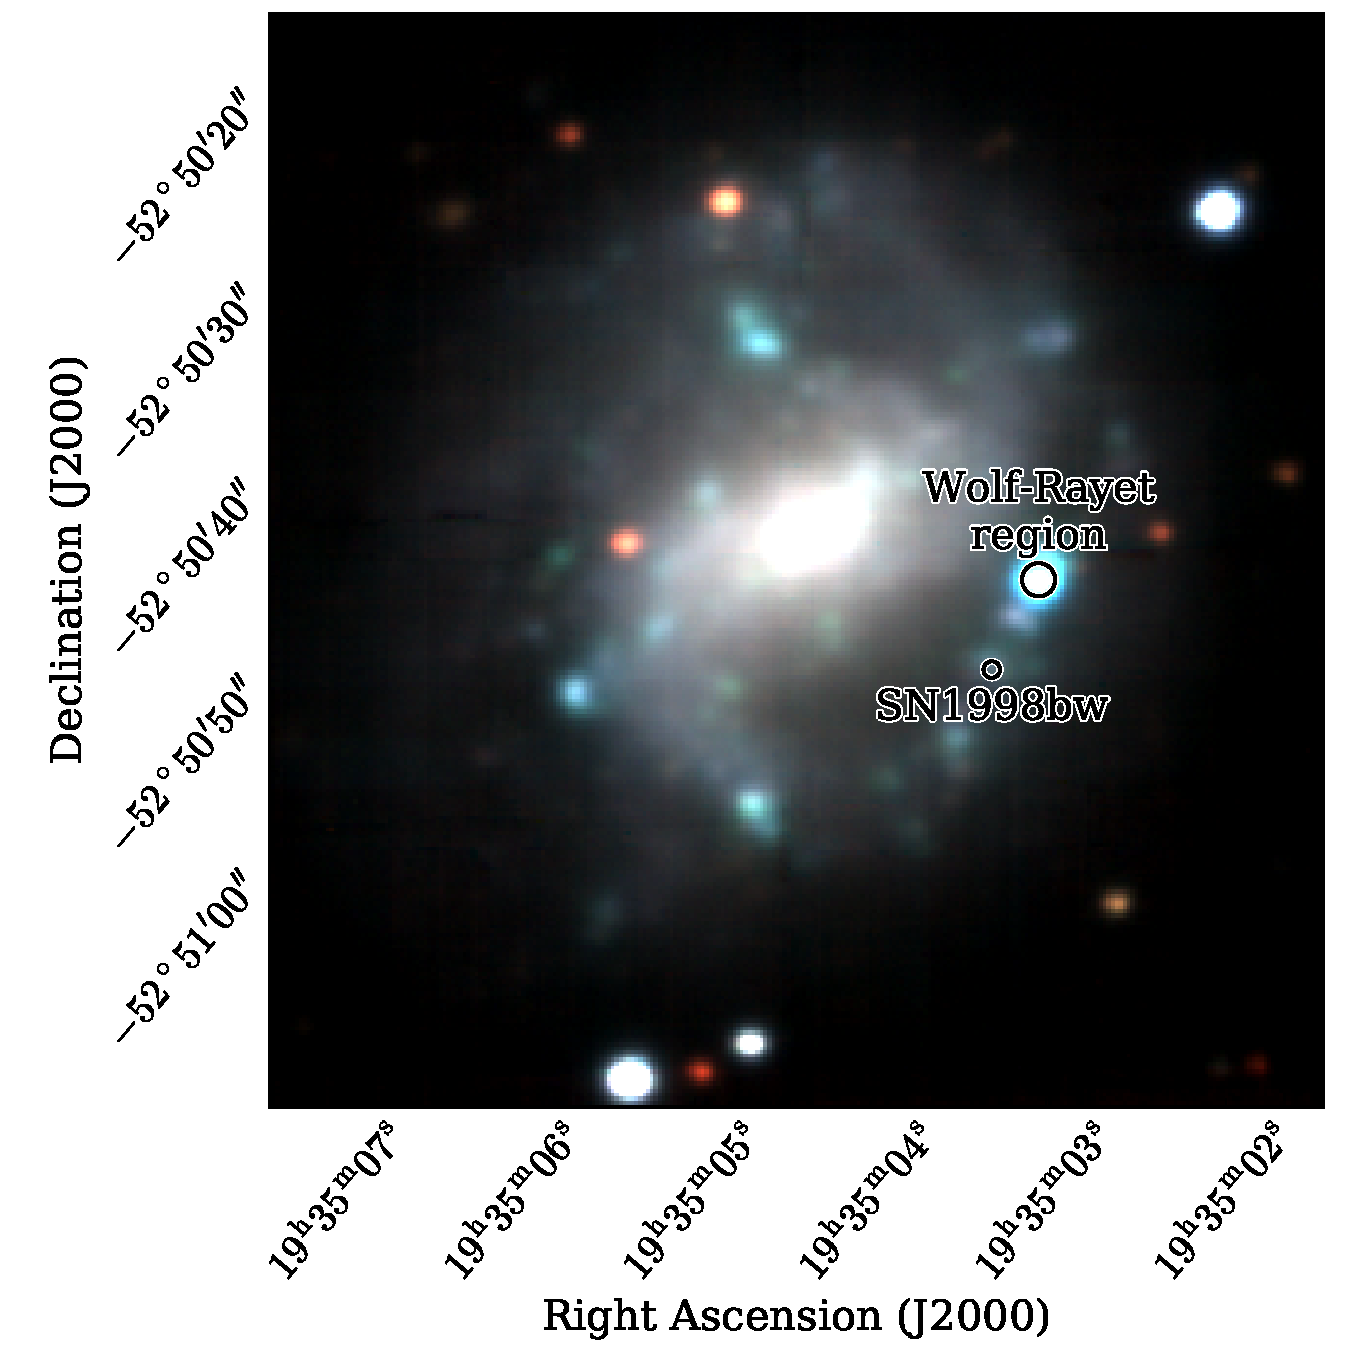
\includegraphics[width=0.990\linewidth]{Figs/MUSE_SN1998bw_RGB.pdf}
\end{subfigure}
\caption{Reconstructed image from the MUSE data cube. False-color composite from reconstructed $VRI$-band images. The image spans approximately 55" by 55", or 10 by 10 kpc. One MUSE spaxel corresponds to 35~pc. The effective spatial resolution is given by the point spread function with a FWHM of approximately 0\farc{9}.}
\label{fig:HaEW}
\end{figure}

The focus of this article are our new observations of the poster-child of the GRB/SN connection, GRB\,980425 or SN\,1998bw obtained with the Multi-Unit Spectroscopic Explorer (MUSE, \citealp{2010SPIE.7735E..08B}). GRB\,980425 is the closest GRB yet discovered and both the GRB \citep[e.g.,][]{1998Natur.395..670G, 1998Natur.395..663K}, the SN \citep[e.g.,][]{1998Natur.395..672I, 2001ApJ...555..900P, 2006ApJ...640..854M} and host galaxy \citep[e.g.,][]{2000ApJ...542L..89F, 2005NewA...11..103S, 2006A&A...454..103H, 2009ApJ...693..347M} are extensively discussed in existing literature. 

Despite the large set of recent literature on the subject, we have decided to summarize our new data and conclusions here mainly because of three reasons: The unique combination of spatial resolution and sensitivity of MUSE helps to clarify some of the ambiguities around SN\,1998bw from previous works. The MUSE data provides the best constraints the immediate environment and underlying stellar population of SN\,1998bw and thus its progenitor yet available. And last but possibly most important, it is an informative example of spatially-resolved oxygen-abundance measurements in star-forming galaxies through strong line diagnostics and their dependence on other physical conditions in the interstellar medium.

The host galaxy of GRB~980425/SN1998bw, ESO184-G82 \citep{1989spce.book.....L}, is a barred spiral dwarf galaxy \citep{2000ApJ...542L..89F} seen nearly face on (Figure~\ref{fig:HaEW}) with a visible extend of approximately 67" by 57" (12 x 10 kpc) at the $B=26.5$~mag isophote \citep{2005NewA...11..103S}. Its brightness, luminosity, and stellar mass are $B=14.94$~mag, $M_B=-17.65$~mag or $L=0.05~\mathrm{L}^{\star}$, and $\log (M_{*}/\mathrm{M}_{\odot})= 8.7 $, respectively \citep{2005NewA...11..103S, 2014A&A...562A..70M}. SN\,1998bw exploded in a \hii-region 12" distant (2 kpc projected) from its center, 860 pc to the South-East from a highly star-forming region which displays strong signatures of Wolf-Rayet stars in its spectrum \citep{2006A&A...454..103H}, the so-called Wolf-Rayet (WR) region (Figure~\ref{fig:HaEW}).

Throughout the paper, we adopt a $\Lambda$CDM cosmology with Planck parameters \citep{2014A&A...571A..16P}, a \citet{2003PASP..115..763C} IMF, and report errors at the 1~$\sigma$ confidence level.

\section{Observations}

We observed ESO184-G82 ($z=0.0086$, or $D_L=37$\,Mpc in concordance cosmology) using the Mulit-Unit Spectroscopic Explorer (MUSE, \citealp{2010SPIE.7735E..08B}) at the VLT on two clear nights starting on 2015-05-14 and 2015-05-15 in a classical observing run from Paranal. In each night, we obtained four dithered exposures of 450~s integration each, totaling 3600~s on source. The on-target frames were supplemented by an offset pointing to blank sky for 200~s. For absolute flux calibration, we observed the spectro-photometric standard LTT3218 at the beginning of each night. The full-width half maximum of the stellar point spread function, which defines our spatial resolution, is between 0\farc{9} (at 9000\,\AA) and 1\farc{1} (at 5000\,\AA) in the MUSE data.

The MUSE instrument is a state-of-the-art integral-field spectrograph (IFS), splitting the light into 24 individual and identical subunits. In the wide-field mode, each of these sub-IFU disperses a $60"\times 2.5"$ region of the sky onto a single CCD. In this way, MUSE covers a continuous sky region of $60"\times 60"$ in the wavelength range between 4800\,\AA\,and 9300\,\AA\, when operated in its nominal configuration. With its excellent total throughput, small spaxel size ($0\farc{2} \times 0\farc{2}$), and decent resolving power ($1800 < R < 3600$ increasing from blue to red wavelengths), MUSE offers a unprecedented combination in sensitivity, spatial resolution and field of view for IFUs \citep{2010SPIE.7735E..08B}.

\section{Data Reduction}

We reduced our data with the pipeline supplied through ESO\footnote{http://www.eso.org/sci/software/pipelines/} in its version \texttt{1.2.1} \citep{2014ASPC..485..451W}, which applies corrections for bias level, flat-fields, illumination level and geometric distortions of MUSE. The ESO pipeline also performs the wavelength calibration using day-time arclamp frames, which is subsequently refined using sky-lines in the science data. The sky background was subtracted using the offset pointing through algorithms from the Zurich Atmospheric Package \citep{2016MNRAS.458.3210S}. The exposures from the two different nights were then corrected for slight pointing offsets between night one and two and stacked using variance-weighting.

The final data cube has slight offsets between the VLT astrometry and a global astrometric solution, which we correct by tying the position of stars in the field of MUSE to coordinates from a reference image taken with the SOFI/NTT on 2000-10-25. We then measure the position of the SN in the reference frame, mapping it onto the MUSE cube with an accuracy of around 50~mas. Figure~\ref{fig:HaEW} shows a broad-band image reconstructed from the MUSE cube where the position of SN\,1998bw is indicated.

In a similar way, we use photometry to corroborate our flux calibration through the $V$, $R_C$ and $I_C$-band magnitudes of star 1 of \citet{2011AJ....141..163C} yielding differences of $0.05\pm0.03$~mag, $0.05\pm0.06$~mag and $0.00\pm0.05$~mag compared to our MUSE spectrum. After applying a small offset using a linear fit to the photometry-based correction factors, we can accurately reproduce the optical colors of the host galaxy \citep{2005NewA...11..103S} to better than 0.02~mag. Before we start deriving physical properties of the host galaxy, we finally de-redden the MUSE data based on the Galactic foreground reddening of $E_{B-V}=0.050$~mag \citep{2011ApJ...737..103S}. 


\section{Analysis and Discussion}

\subsection{Separating gas-phase and stellar component.}

\begin{figure}
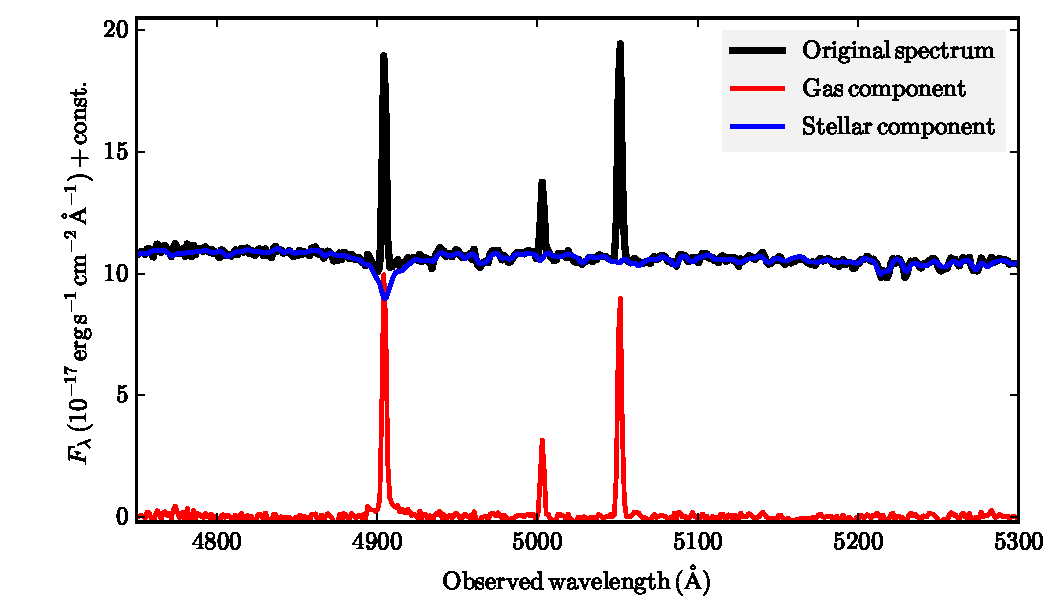
\includegraphics[angle=0, width=0.99\columnwidth]{Figs/Stargas_spec.pdf}
\caption{Separating stellar and gas-phase spectra. This figure shows a zoom-in to the wavelength region around \hb\,including the two strong \oiii($\lambda\lambda4959,5007$) lines at an arbitrary location from the MUSE cube. Black is the original spectrum, blue the fitted stellar component, and red the resulting spectrum for the gas-phase only. Blue and black spectra are shifted to enhance clarity in the Figure. Note the significant Balmer absorption around \hb.}
\label{fig:stargas}
\end{figure}

As we are primarily interested in the absolute and relative strengths of the nebular lines, and thus the gaseous component of the galaxy, we need to remove the stellar component for accurate line flux measurements, in particular for the Balmer lines. The stellar Balmer absorption has a significant influence on the emission line measurement of \hb\, (Figure~\ref{fig:stargas}). It is primarily a function of line intensity and age of the underlying stellar population, and thus depends on the position within a galaxy, and needs to be accurately modeled for reliable constraints on the Balmer decrement.

We separate the galaxy's star and gas components by fitting a linear superposition of template stellar spectra based on the \citet{2003MNRAS.344.1000B} models to the MUSE data. We divide the full field of view into regions with a size of 0\farc{6}x0\farc{6} (or 3 by 3 spaxels), and extract spectra for each of the $\sim9000$ subregions. These spectra are then fit with stellar models using \texttt{starlight} \citep{2005MNRAS.358..363C, 2009RMxAC..35..127C} in a similar fashion as we did elsewhere \citep{2016MNRAS.455.4087G, 2016arXiv160703446K, 2016arXiv160900013P}. The 3x3 co-adding effectively is an increase in signal-to-noise at the expense of spatial resolution for the stellar properties, but is necessary to robustly perform an automated fit in particular in the fainter regions of the galaxy. We then linearly scale the best-fit stellar template to the intensity in single spaxels. Subtracting this stellar component from the original data results into the contribution of the gas-phase only. Figure~\ref{fig:stargas} illustrates this procedure.


\subsection{Equivalent width maps}
\begin{figure}
\begin{subfigure}{.24\textwidth}
  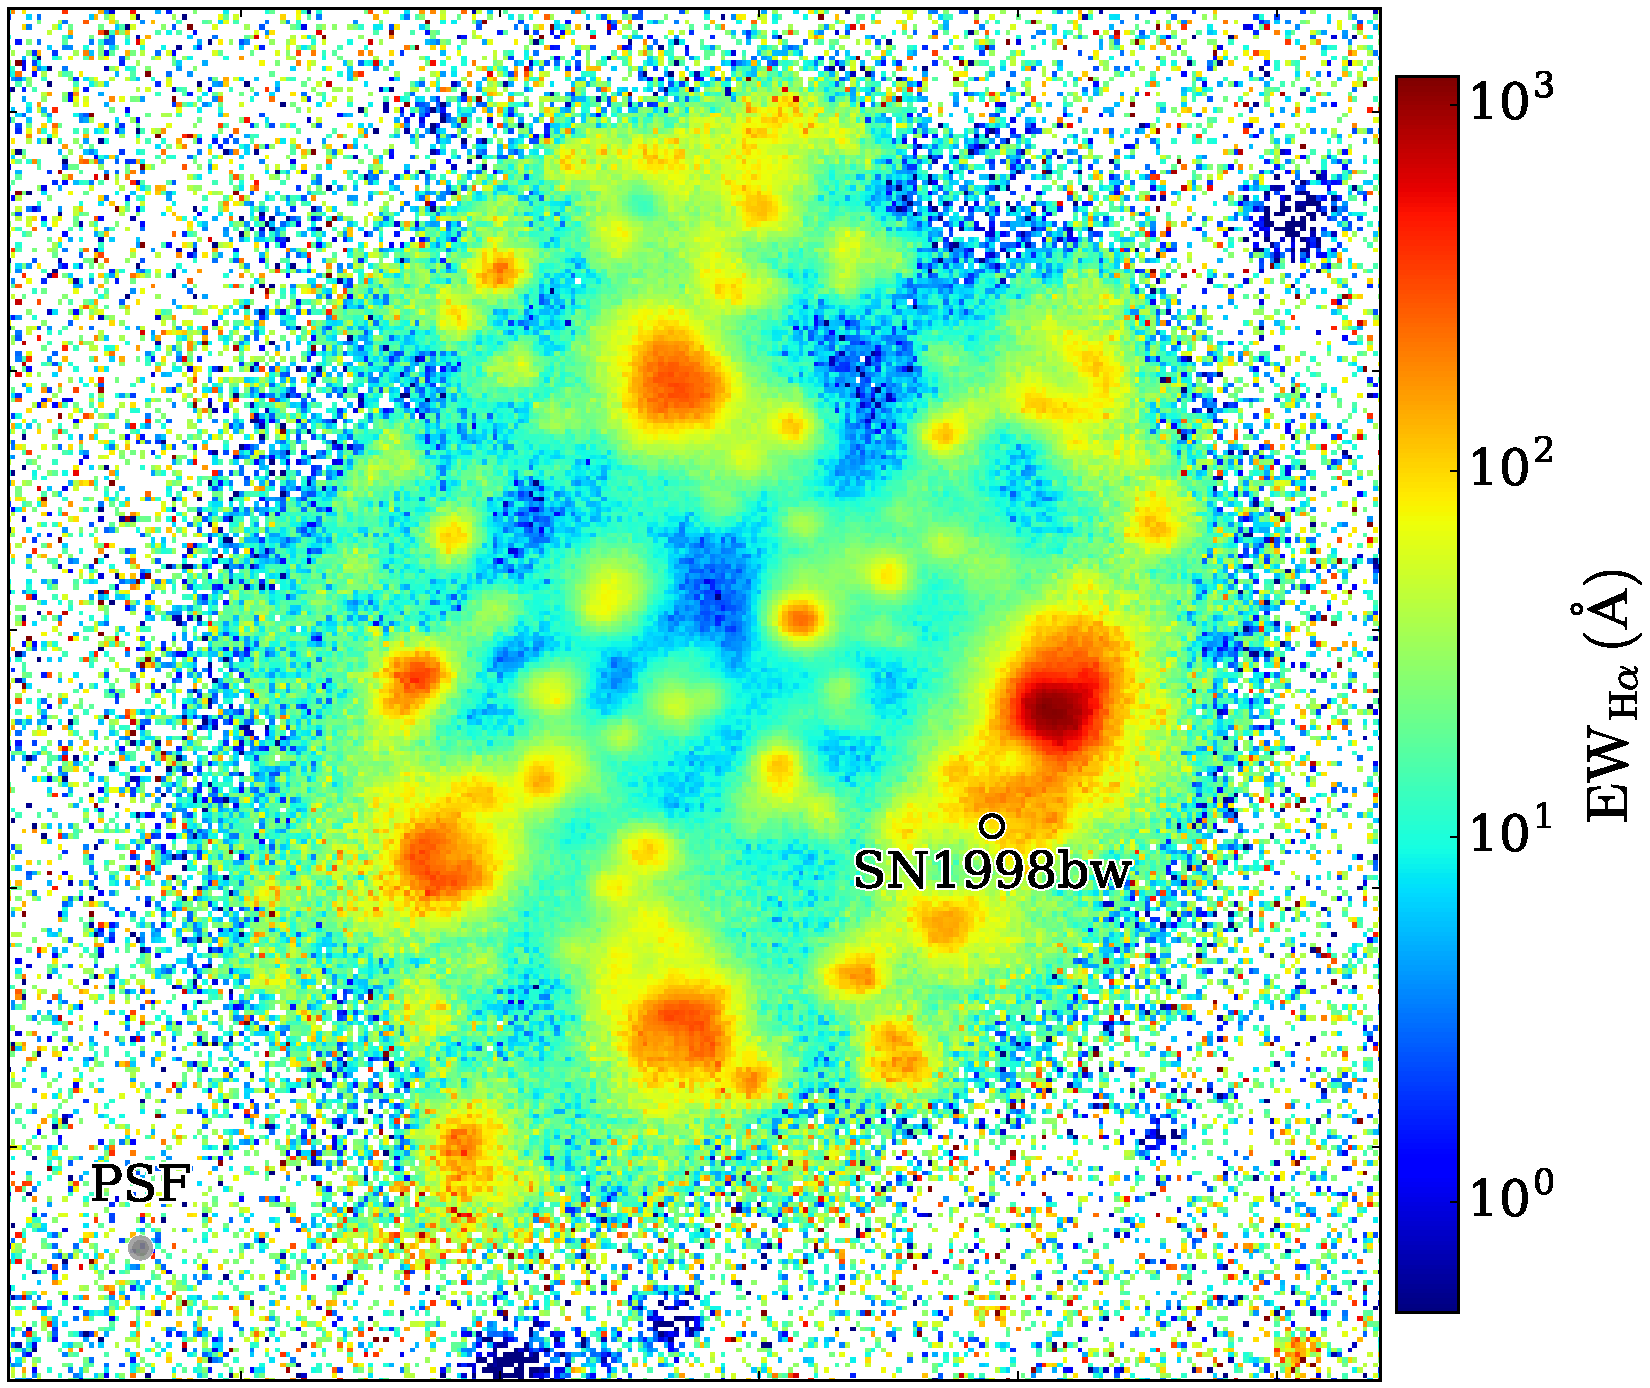
\includegraphics[width=1.0\linewidth]{Figs/MUSE_SN1998bw_HaEW.pdf}
\end{subfigure}
\begin{subfigure}{.24\textwidth}
  \hspace*{-0.1cm}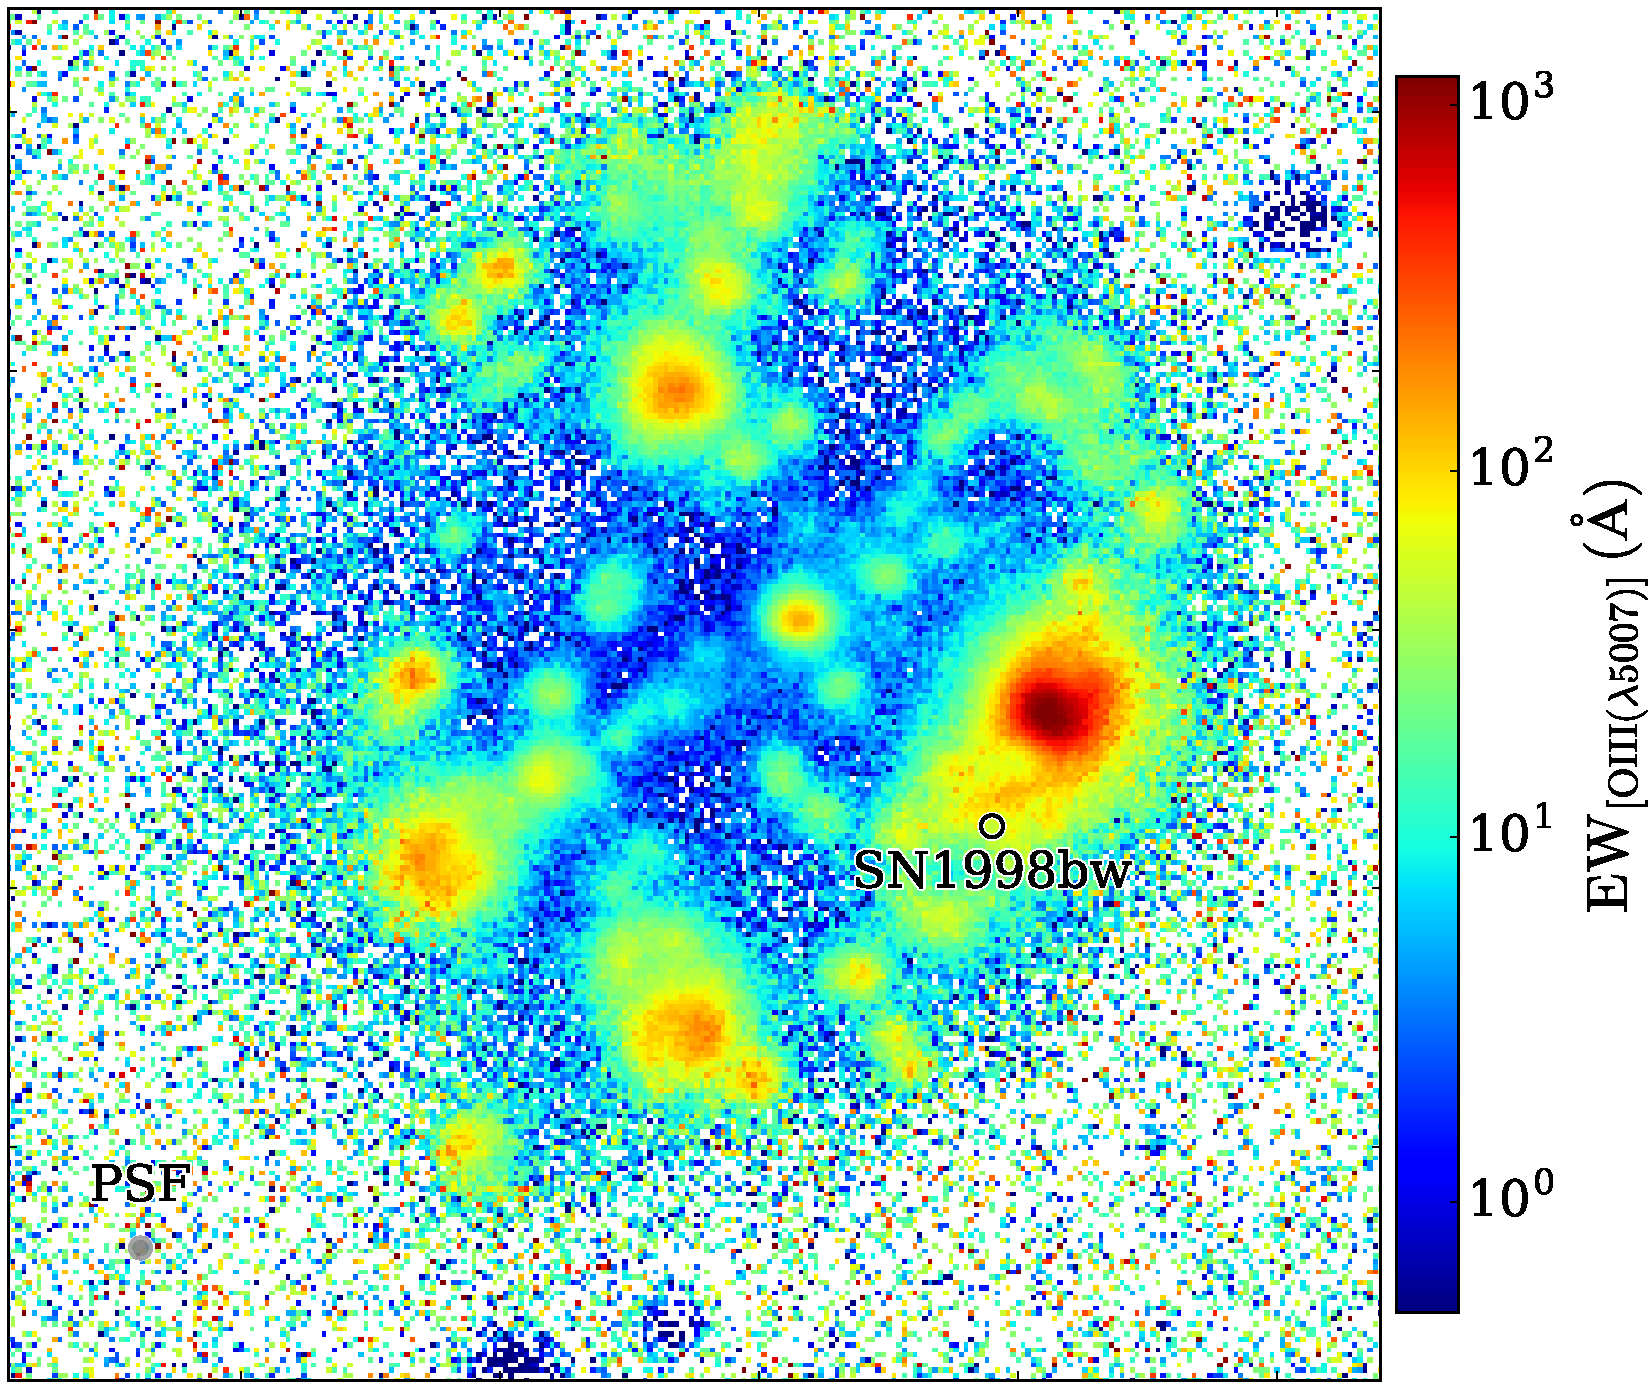
\includegraphics[width=1.0\linewidth]{Figs/MUSE_SN1998bw_OIIIEW.pdf}
\end{subfigure}
\begin{subfigure}{.24\textwidth}
  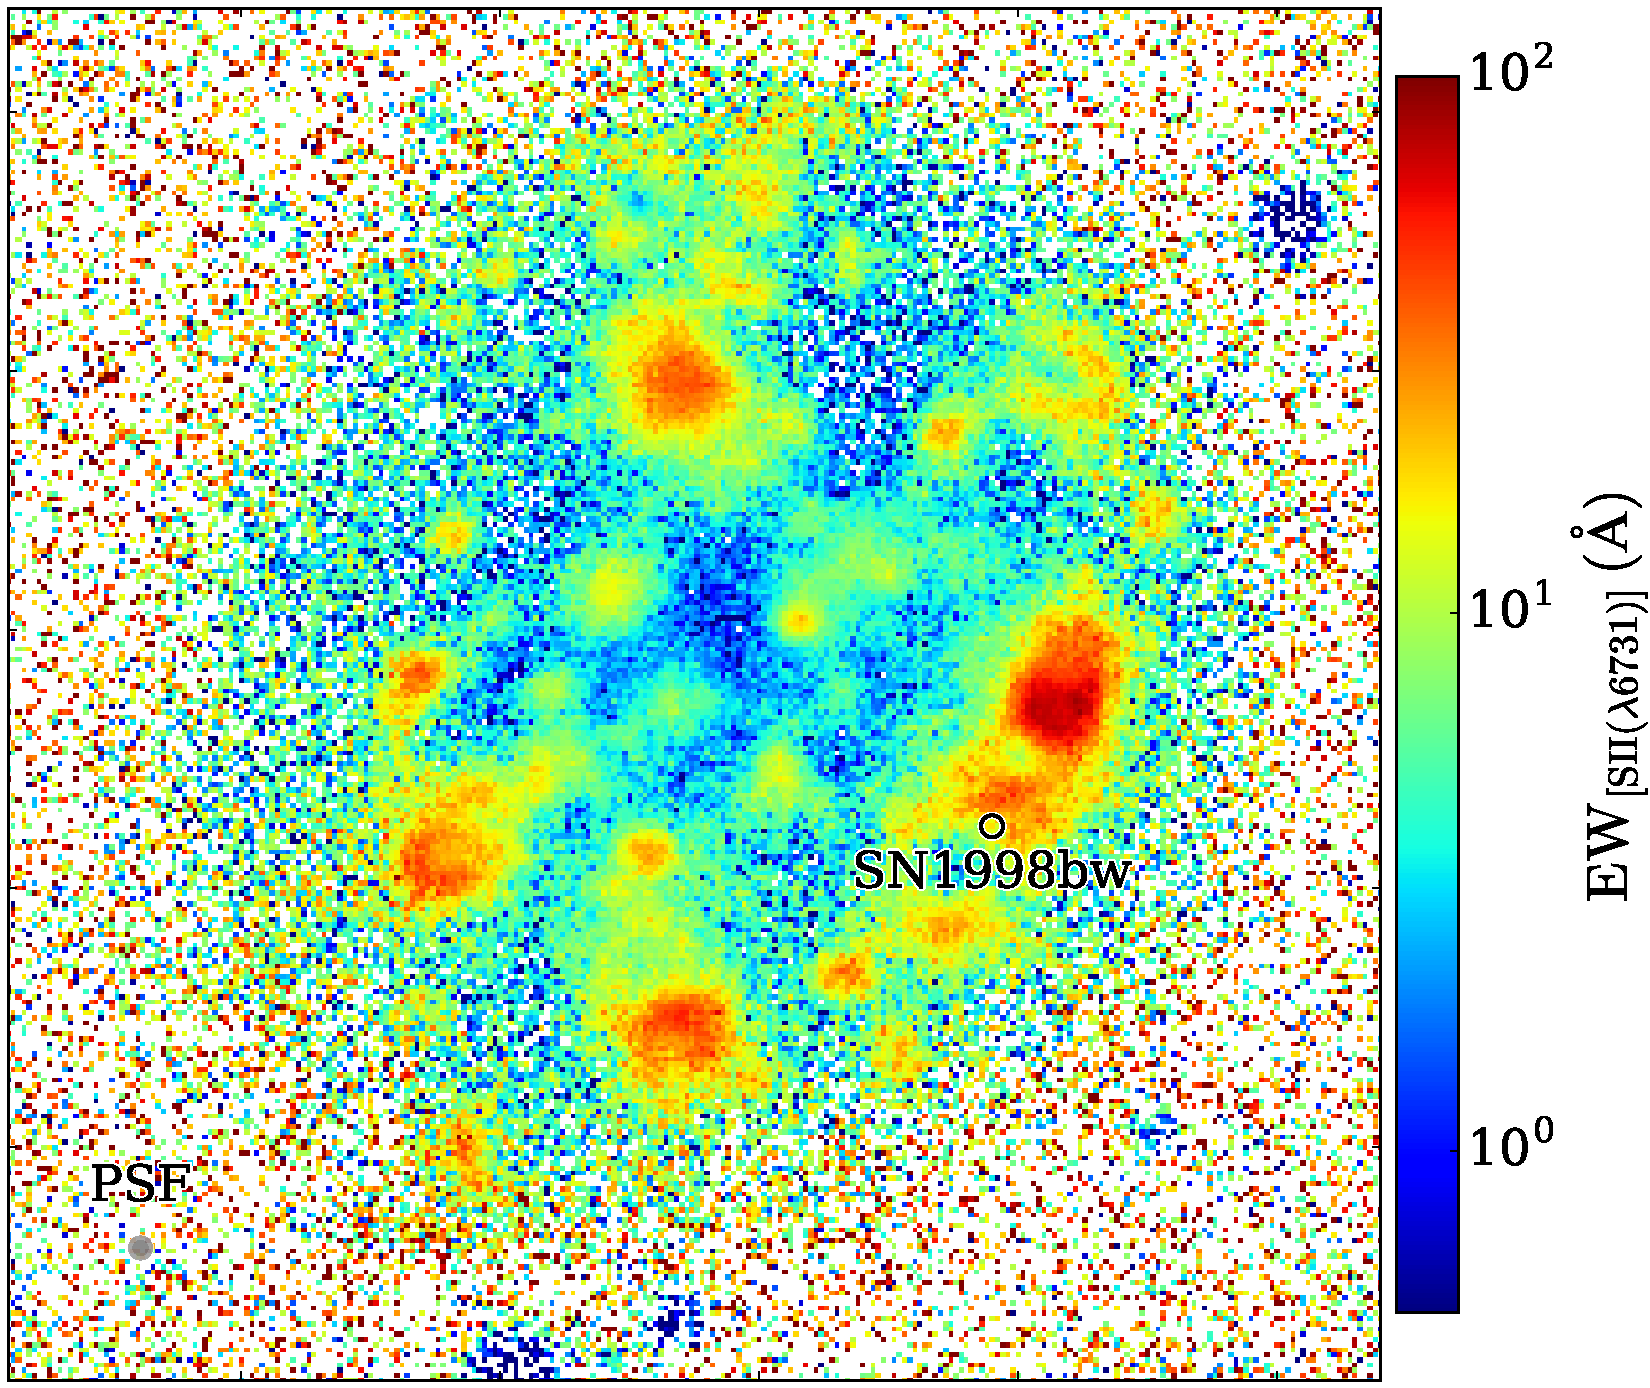
\includegraphics[width=1.0\linewidth]{Figs/MUSE_SN1998bw_SIIEW.pdf}
\end{subfigure}
\begin{subfigure}{.24\textwidth}
  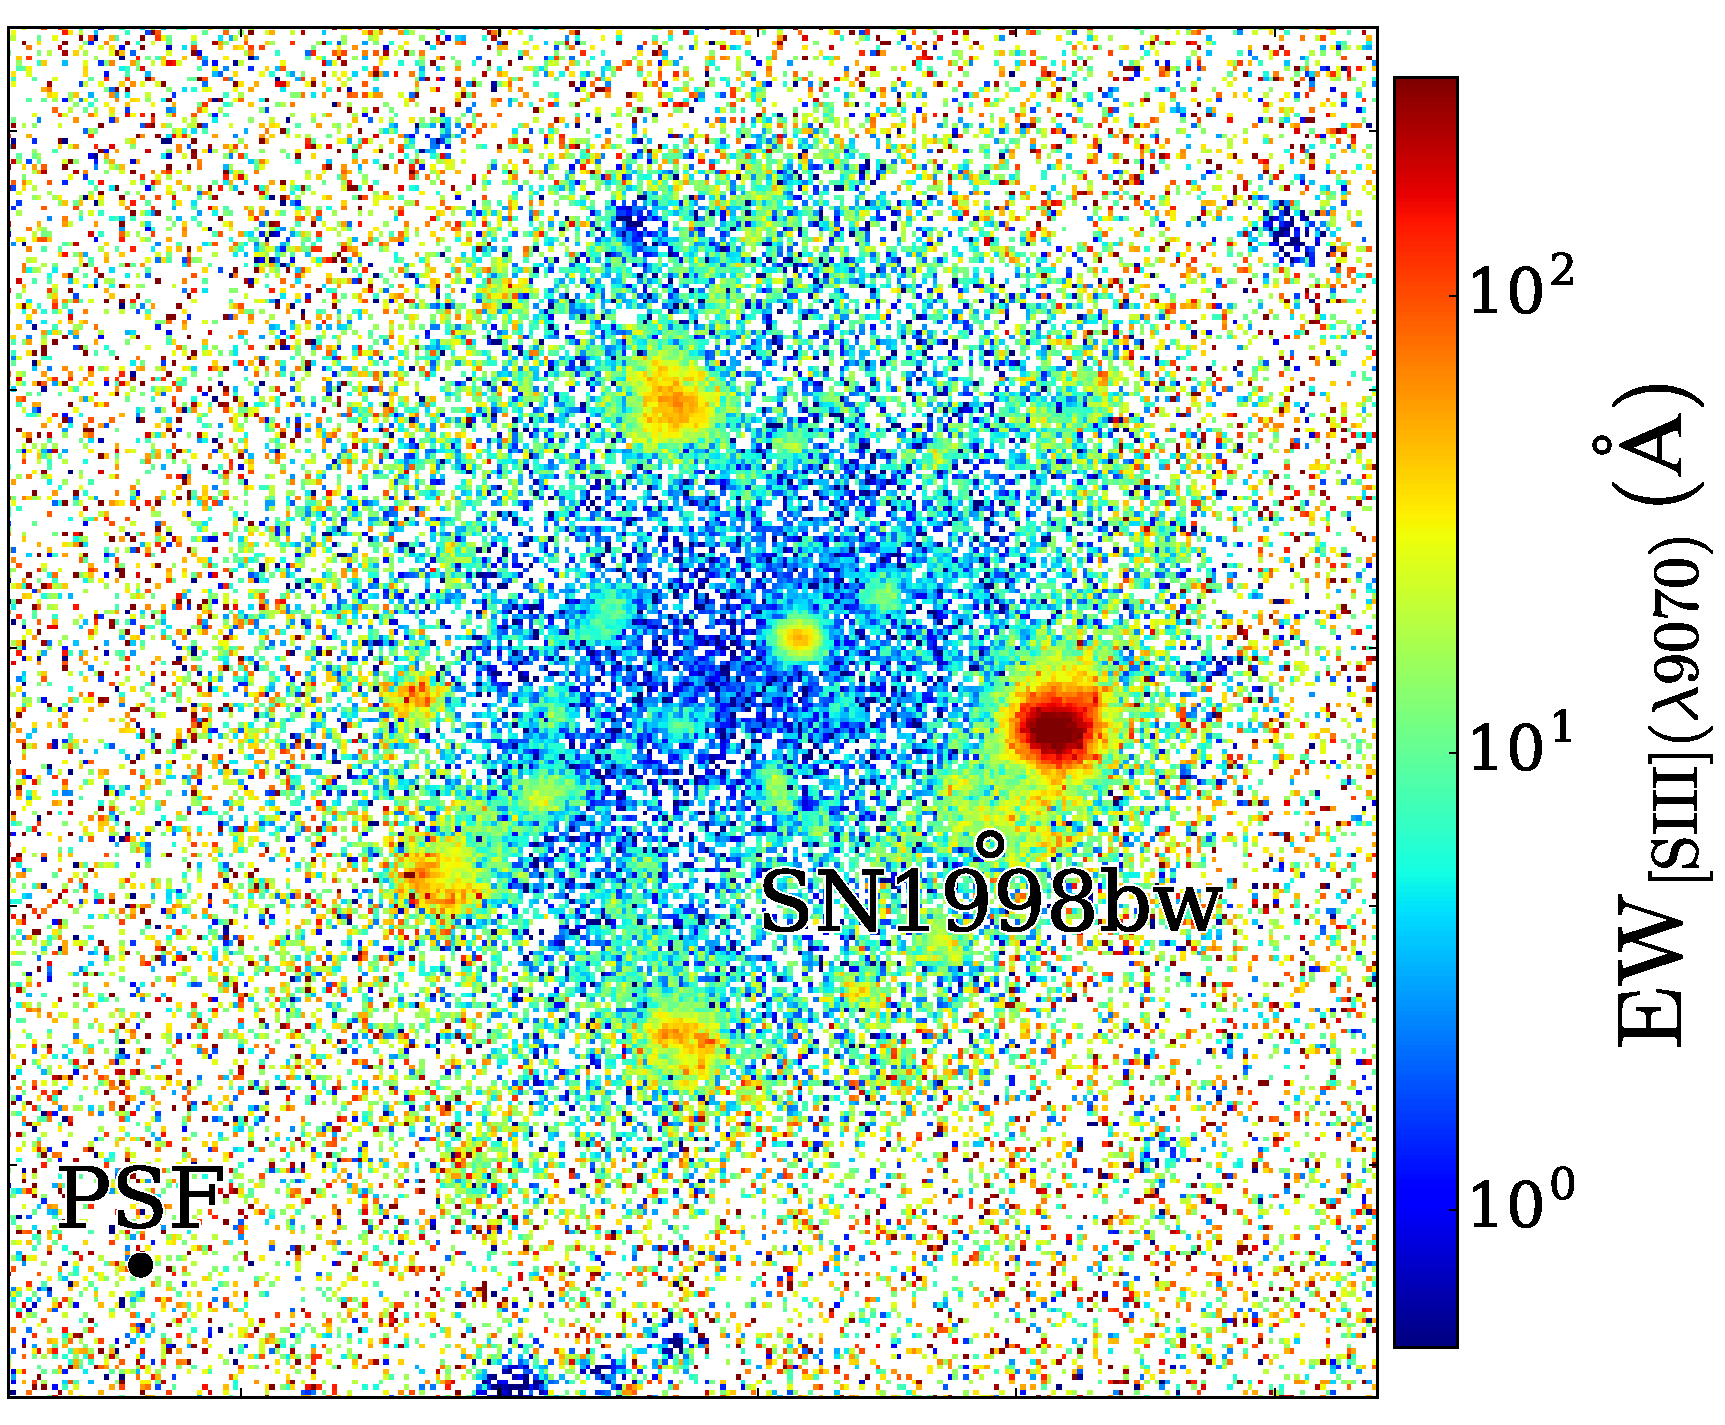
\includegraphics[width=1.0\linewidth]{Figs/MUSE_SN1998bw_SIIIEW.pdf}
\end{subfigure}
\caption{Reconstructed images from the MUSE data cube. Each panel shows the host of GRB~980425 in a different wavelength regime. Top-left: \ha, top-right: \oiii($\lambda$5007), bottom-left: \sii($\lambda$6731), bottom-right \siii($\lambda$9070). All panels are approximately 55" by 55", or 10 by 10 kpc in size. One MUSE spaxel corresponds to 35~pc. The effective spatial resolution is given by the point spread function indicated in the lower left corner of each image with a FWHM of approximately 0\farc{9}.}
\label{fig:EW}
\end{figure}

After having separated gas-phase and stellar component it is trivial to produce maps of line flux (integral over the gas-phase component), continuum (average of the stellar component) and equivalent width (flux divided by continuum). Figure~\ref{fig:HaEW}~displays the \ha\,equivalent width map, which is a rather direct proxy of stellar population age, which then can be interpreted as a tracer for progenitor mass. %A comparison with the similar figure derived using the previous generation of IFUs \citep[Figure 4 in][]{2008A&A...490...45C} illustrates the impressive gain that MUSE offers in terms of spatial resolution and sensitivity over the previous generation of IFUs. 
The spaxel closest to the SN/GRB position has an \ha\,equivalent widths of EW=98\,\AA. The spaxels within a radius of 70 pc yield EW$_{\mathrm{H\alpha}}=88\pm15$\,\AA. 

Assuming a single stellar population from an instantaneous starburst, this corresponds to stellar-population ages between 5.5 Myr and 9 Myrs from various models at metallicities of $Z=0.004$ or $Z=0.2$\,Z$_{\odot}$ \citep[see e.g.,][and references therein]{2016arXiv160703446K}. The relatively large range in ages is almost entirely due to the spread from different stellar evolution models. These ages corresponds to life-times of stars with zero-age main sequence masses (ZAMS) of approximately 20 to 40~M$_{\odot}$ \citep{1994A&AS..105...29F, 2005A&A...429..581M}, which is similar to the one derived by modeling the SN\,1998bw nebular spectra of $M_{\rm{ZAMS}} \gtrsim 30-35$\,M$_{\odot}$ \citep{2006ApJ...640..854M} or found previously from host spectra \citep{2005NewA...11..103S}.

These considerations are only valid, of course, if the progenitor was born where it exploded, and was not kicked out of the nearby WR region, for example \citep{2006A&A...454..103H}. However, very high EW values of \ha~and nebular transitions are observed in the center of the WR-region (both EW$_{\mathrm{H\alpha}}$ and EW$_{\oiii}>1000$). Together with the detection of strong \hei($\lambda4922$), they correspond to star-burst ages of around 3 Myr or less in instantaneous star-burst models, or $M_{\rm{ZAMS}} \gtrsim 60$\,M$_{\odot}$ \citep[see e.g.,][and references therein]{2015MNRAS.451L..65T}. The discrepancy with respect to the progenitor mass from SN modeling suggests, however, that the GRB progenitor was not formed in the WR-region, but rather formed in situ. The scenario of ejection from the nearby Wolf-Rayet region at a projected distance of 860 pc \citep{2006A&A...454..103H} appears contrived\footnote{The spatial association of the SN position with another, fainter \hii-region would be coincidental in that scenario.}. For a travel time shorter than the age $\tau$ of the Wolf-Rayet region ($\tau<3$\,Myr), the required peculiar velocities $v$ are extremely high ($v>260\,\mathrm{km\,s^{-1}}$). Projection effects would further increase the required velocities. Scenarios that are believed to give rise to runaway stars are dynamical few-body encounters or binary supernovae, but both seem unfeasible here: A dynamical ejection produces hyper-velocity stars in only very rare and extreme cases \citep{2001A&A...365...49H, 2012ApJ...751..133P}, and the probability of potential GRB progenitors ($M_{\rm{ZAMS}}\gtrsim 20\,M_\odot$) getting velocity kicks with $>200\,\mathrm{km\,s^{-1}}$ from a companion SN is also practically zero \citep{2011MNRAS.414.3501E}. The young age of the Wolf-Rayet region is an additional constraint. It makes a binary supernova origin highly implausible as there would not be enough time to evolve and explode the primary and eject the secondary to a distance $\gtrsim860$\,pc. Also the fraction of ejected stars by dynamical encounters is of course a function of the elapsed time, and reaches only 0.01/0.03 at 1 or 3 Myr at $M_{\rm{ZAMS}}\sim 35\,M_\odot$ \citep{2012ApJ...746...15B}, again leaving little time for the ejected star to travel as far as 860 pc (or further).

Given the presence of massive stars in the vicinity of the SN position \citep{2000ApJ...542L..89F}, the substantial level of star-formation as evidenced through high EW of nebular lines at the SN position (Figure~\ref{fig:EW}), and the consistency between $M_{\rm{ZAMS}}$ derived from the age of the stellar population as well as the SN~1998bw nebular spectra, we see no compelling reason to invoke an artificial ejection from the nearby WR region to explain the GRB location within its host.

\subsection{Dust distribution}

\begin{figure}
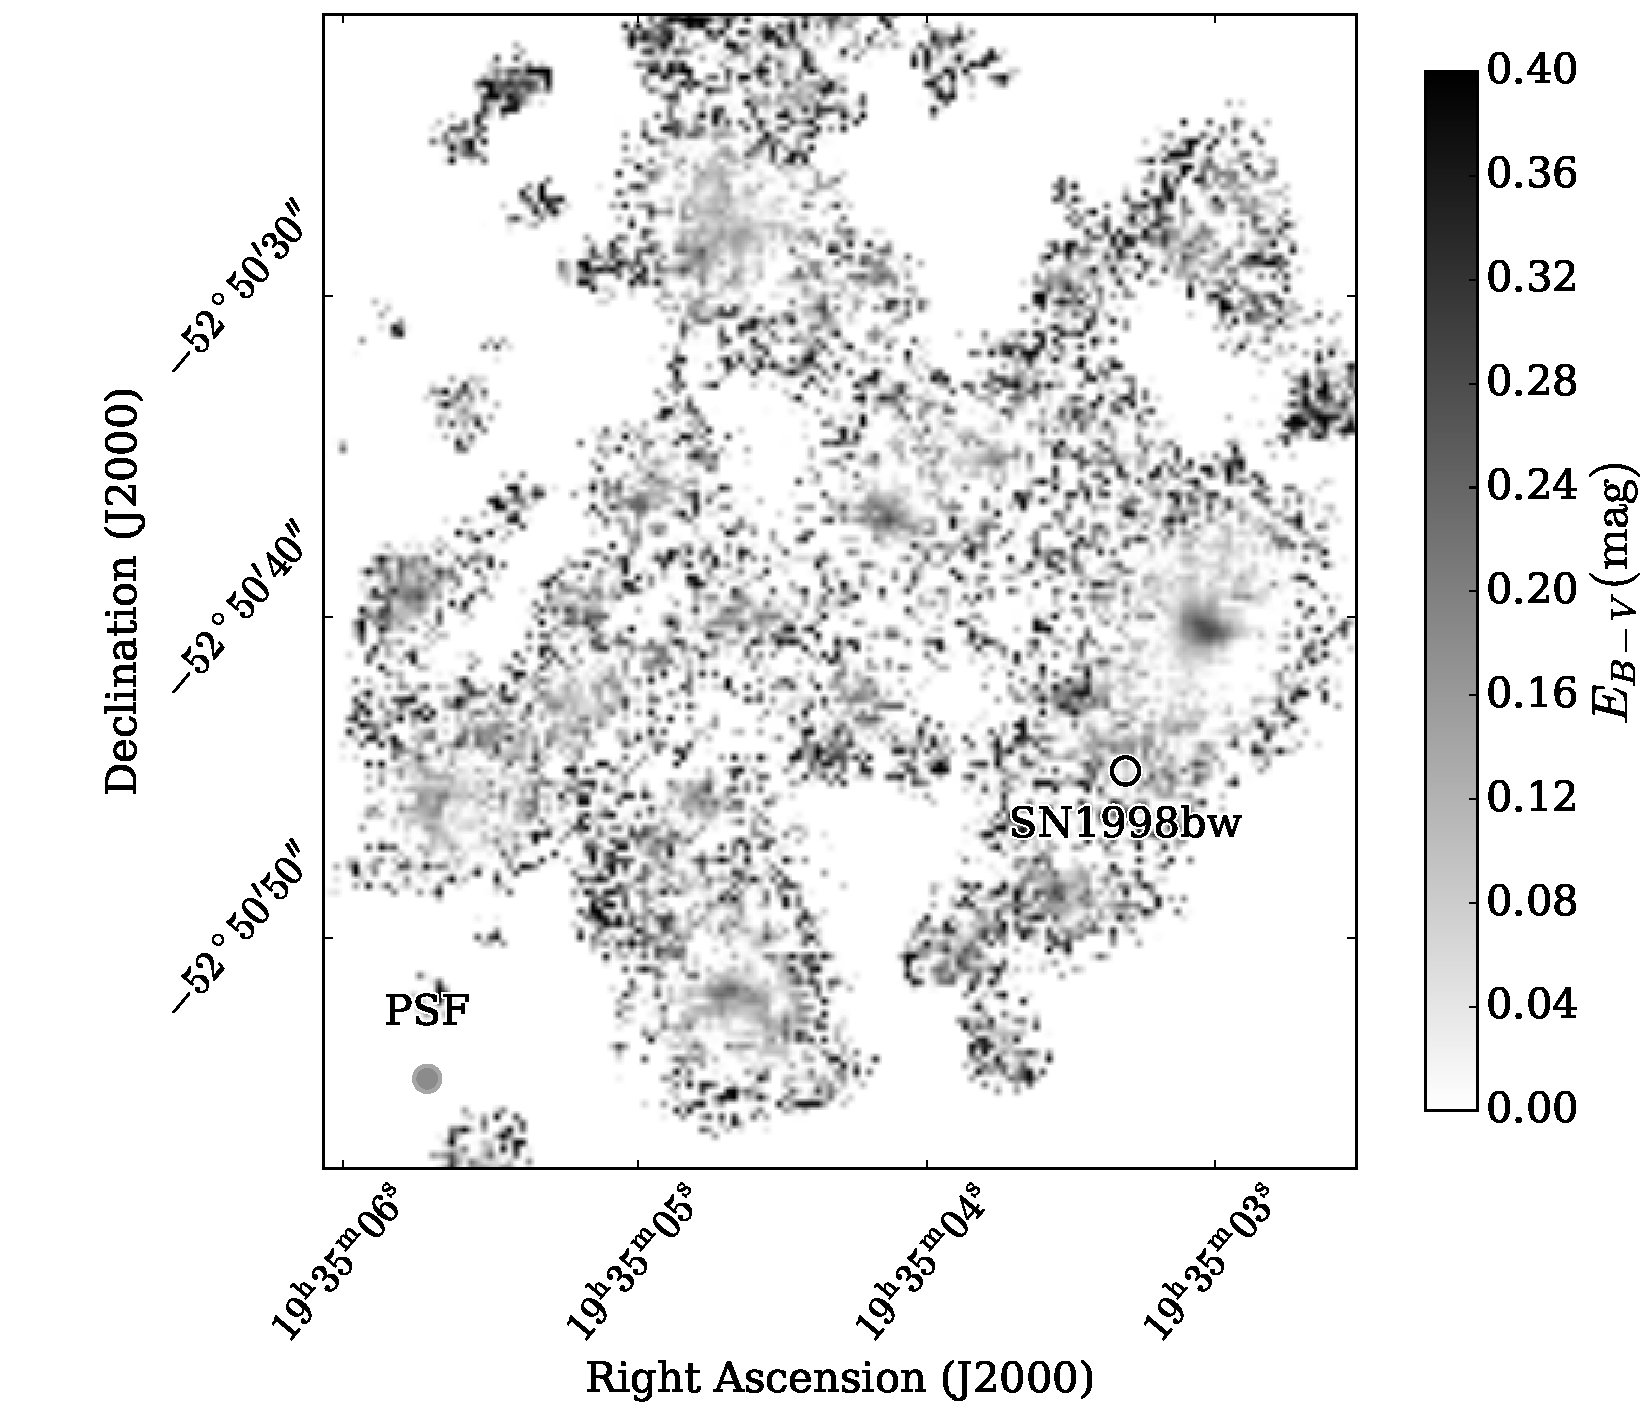
\includegraphics[angle=0, width=0.99\columnwidth]{Figs/MUSE_SN1998bw_EB-V.pdf}
\caption{Dust distribution in ESO184-G82 as measured through the Balmer decrement. We only show spaxels in which \hb\, is detected with a significance of at least 3~$\sigma$. The shown image spans 34" by 38", or 6.1 by 6.8 kpc. The circle denoting the position of SN\,1998bw has a radius of 180 pc.}
\label{fig:ebv}
\end{figure}

A further physical quantity of interest is the amount and distribution of dust at the SN position as probed by the Balmer decrement. Because of its exquisite photometric and spectroscopic data set, SN1998\,bw is a widely-used comparison object, so it is fundamental to understand whether the SN was dust reddened to derive its intrinsic properties. We convert our line fluxes of \ha\,and \hb\, into a map of color-excess $E_{B-V}$ using the Milky-Way extinction law as shown in Figure~\ref{fig:ebv} using Equation 5 of \citet{2015A&A...581A.125K}. This procedure assumes standard ratios of the Balmer lines at $10^4$\,K and $n_e\sim100\,\mathrm{cm}^{-3}$ from \citet{1989agna.book.....O}, broadly consistent with the values obtained for this galaxy (Table~\ref{tab:prop}). Our results depend only marginally on the specific choice of the extinction law, as the difference between reddening laws in the local group is small in the wavelength range probed by \ha\, and \hb. 

Figure~\ref{fig:ebv}~shows very little dust in general in ESO184-G82, and also only minor evidence for dust at the actual GRB/SN position ($E_{B-V} = 0.06\,\mathrm{mag}$, or $A_V = 0.19\,\mathrm{mag}$) and its immediate environment $E_{B-V} = 0.03_{-0.03}^{+0.06}\,\mathrm{mag}$ in the 9 spaxels closest to the GRB/SN position). The only location that show evidence for significant dust reddening are the centers of \hii\, regions as exemplified by the WR-region, which shows a centrally-symmetric subtructure in dust extinction decreasing from the inside out peaking at $E_{B-V} \sim 0.3\,\mathrm{mag}$ or $A_V = 0.9\,\mathrm{mag}$. A galaxy-integrated spectrum yields $E_{B-V} = 0.05\pm0.02$~mag, or $A_V=0.15\pm0.06$~mag, which is in remarkable agreement with the average optical depth $\tau_V$ derived from modeling the UV-to-radio SED \citep{2014A&A...562A..70M}.

These values are in tension to the significant values of dust reported previously using other spectra \citep{2006A&A...454..103H, 2008A&A...490...45C, 2009ApJ...691..182S}. It is not immediately clear what causes the disagreement in particular to the spatially-resolved data of \citet{2008A&A...490...45C}. The tension, however, is lowest/highest in regions of high/low \hb\, equivalent width, and we speculate that an under-correction of the stellar Balmer absorption at \hb\, in \citet{2008A&A...490...45C} could lead to a lower \hb\, flux measurement and thus an overestimated \ebv~value and might explain the observed behavior.

Negligible amounts of dust at the location of SN\,1998bw have been derived from optical host spectra already in \citet{2005NewA...11..103S}. The dust distribution, with the only significant detection at the centre of the WR-region is consistent with that inferred from the spatially-resolved, long-wavelength observations \citep{2014A&A...562A..70M}. The latter report little dust obstruction in general for the galaxy, and a concentration of the IR, millimeter and radio emission at the position of the WR-region. Also quantitatively, our measurements of the visual extinction $A_V$ in the WR region and galaxy-integrated are remarkably consistent with the UV-to-radio modeling of \citet{2014A&A...562A..70M}.

Our new data thus resolve the apparent conflict with the unexpectedly large reddening at the SN position derived from previous spectroscopic data \citep{2006A&A...454..103H, 2008A&A...490...45C} and the SN itself, which did not show any evidence of strong dust obscuration \citep[e.g.,][]{1998Natur.395..672I, 2001ApJ...555..900P}. They provide further confidence in using SN\,1998bw as an only very mildly reddened SN template for comparison to other events \citep[e.g.,][and numerous references therein]{2004ApJ...609..952Z, 2016arXiv160606791K}.

\subsection{Metallicity Diagnostics}

\subsubsection{Initial considerations}

\begin{figure}
\begin{subfigure}{.24\textwidth}
  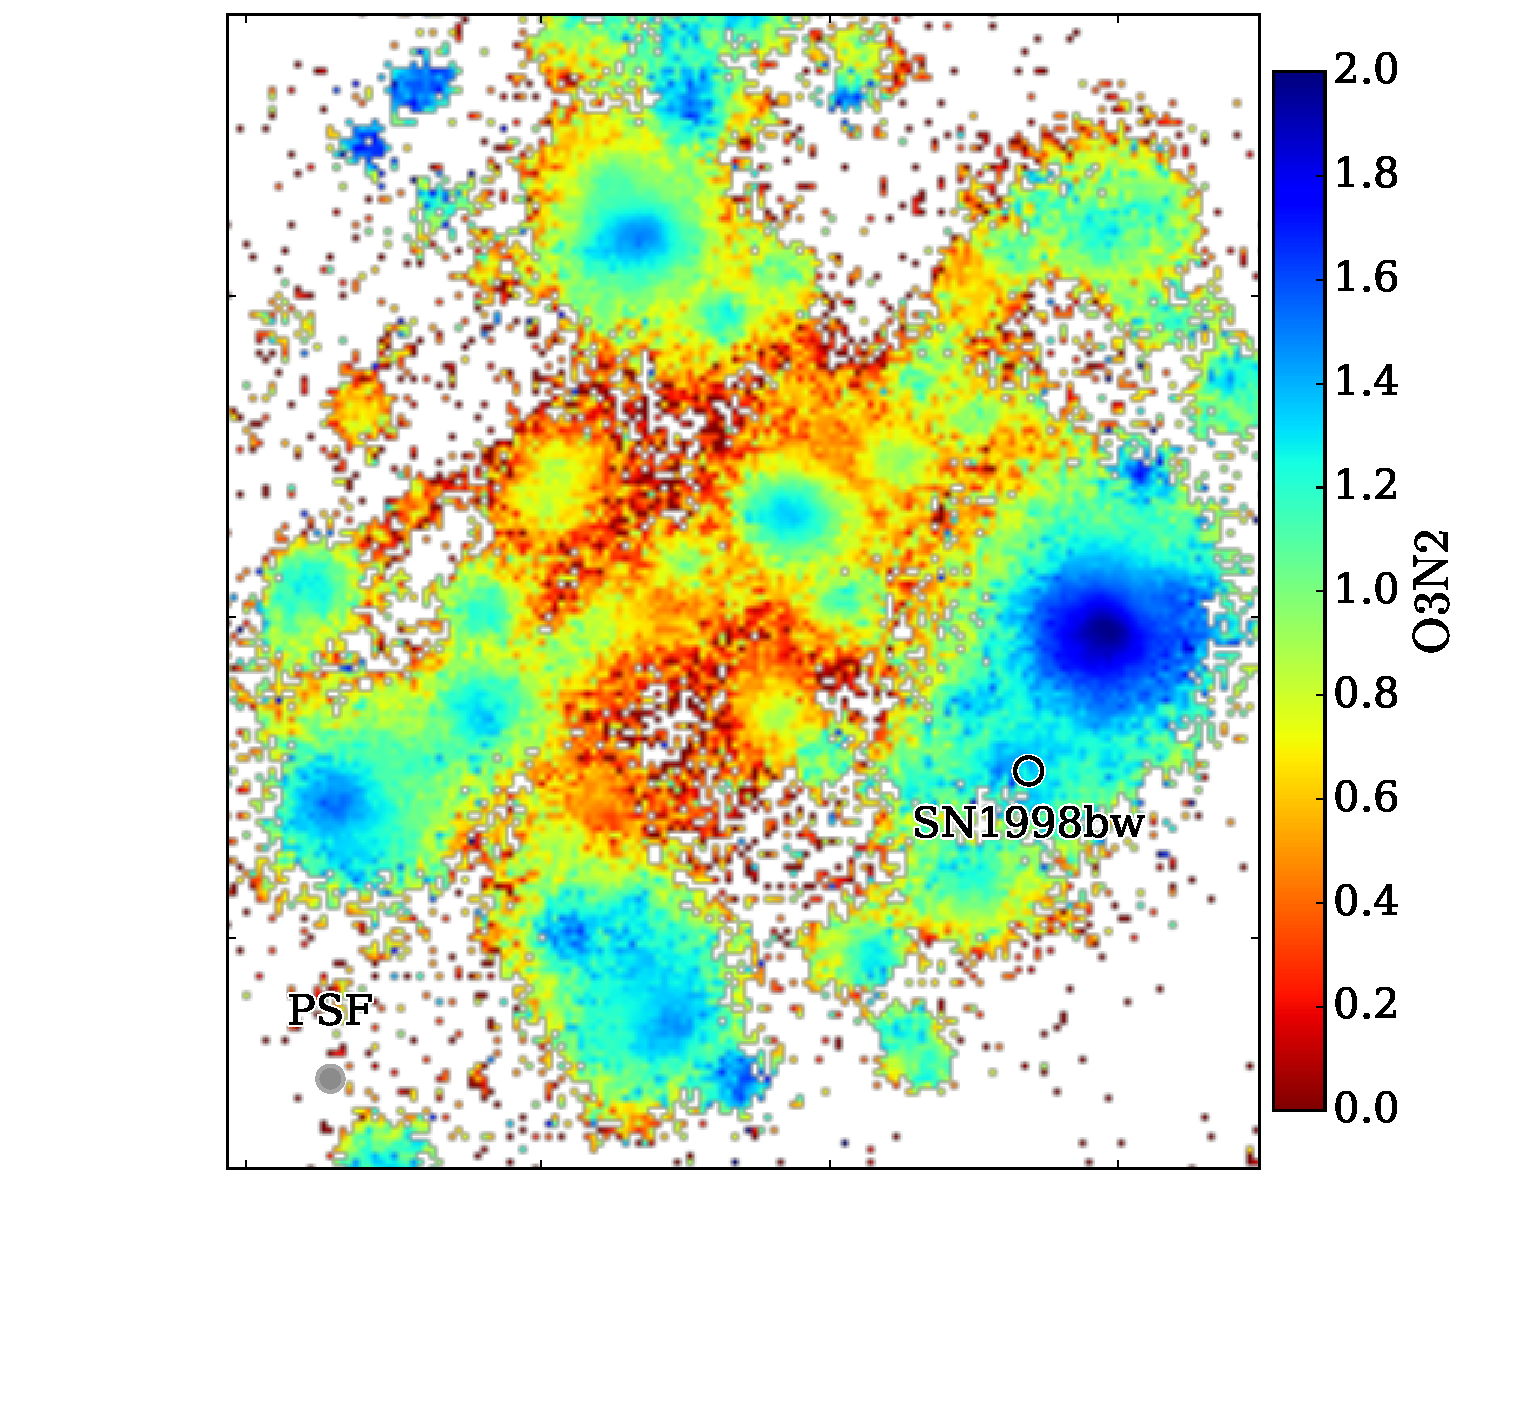
\includegraphics[width=0.999\linewidth]{Figs/MUSE_SN1998bw_O3N2.pdf}
\end{subfigure}
\begin{subfigure}{.24\textwidth}
  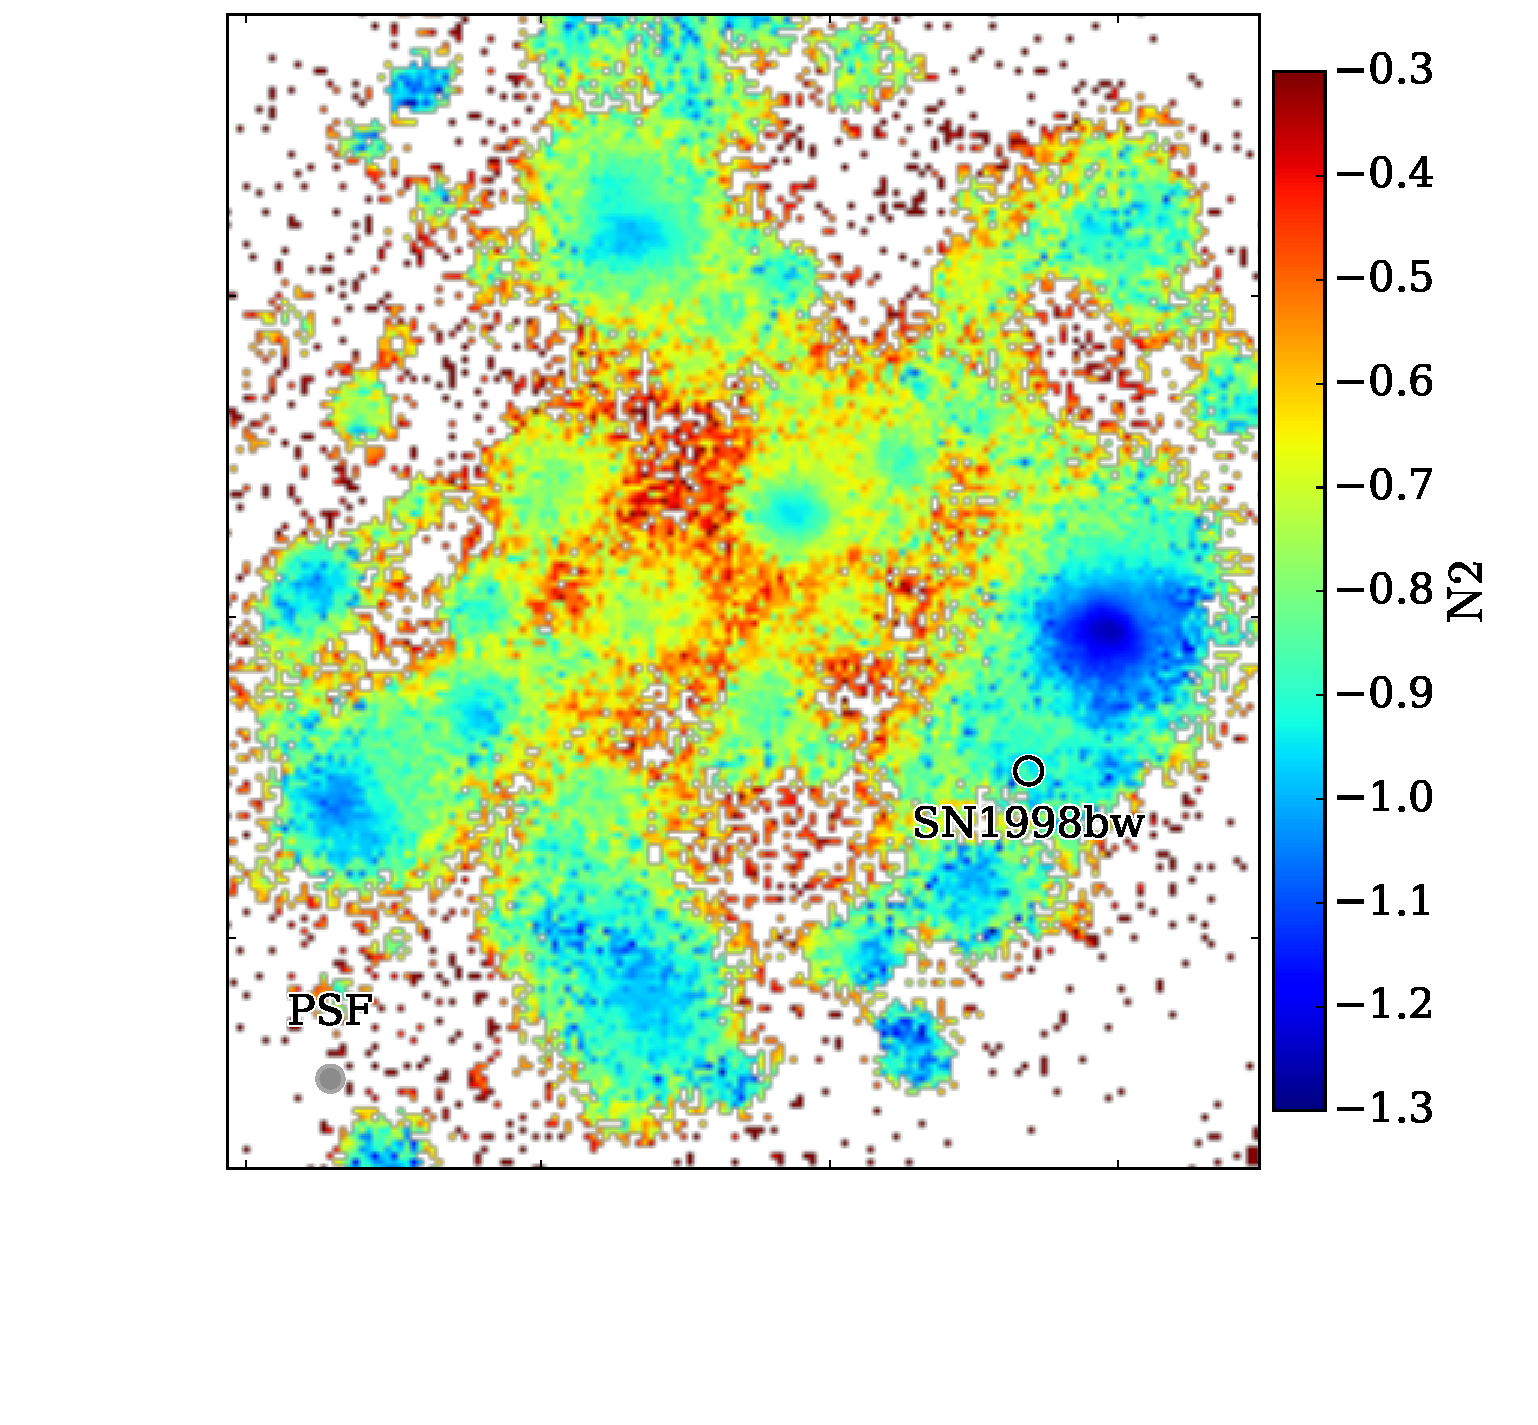
\includegraphics[width=0.999\linewidth]{Figs/MUSE_SN1998bw_N2.pdf}
\end{subfigure}
\caption{Maps of O3N2 and N2. Only spaxels with a combined signal-to-noise ratio of at least three are shown. In the O3N2 and N2 strong line diagnostic, low oxygen abundances correspond to blue/red colors (N2=-1.2/-0.9 or  O3N2=1/1.6 would translate to \oh=8.2/8.4, respectively). Individual \hii-regions show strong radial symmetric sub-structure in both line ratios. Image dimensions are similar to Figure~\ref{fig:ebv}.}
\label{fig:o3n2}
\end{figure}

Metal abundances in \hii\,regions are a central observable to study cosmic chemical evolution, and a large set of literature is devoted to the various possibilities, their advantages, and perils to infer abundances from \hii-region spectra  \citep[e.g.,][]{1979MNRAS.189...95P, 1991ApJ...380..140M, 2005ApJ...631..231P, 2008ApJ...681.1183K}. Very briefly, the most common methods to infer chemical abundances, and from those, the abundance of oxygen (traditionally expressed in \oh) make use of either photo-ionization models \citep[e.g.,][]{1985ApJS...58..125E, 2000ApJ...542..224D, 2002ApJS..142...35K} or empirical correlations between certain strong-line ratios and oxygen abundances derived through electron temperatures $T_{\rm{e}}$ from collisionally-excited lines \citep[CELs, e.g.,][]{2004MNRAS.348L..59P, 2013A&A...559A.114M}. Commonly used ratios are for example \nii/\oii, \oiii/\nii, \nii/\ha, or $R_{23}$ = (\oii+\oiii)/\hb, which have been (re)-calibrated numerous times against different samples of $T_{\rm{e}}$ or photo-ionization models, yielding a large set of different calibrators in the literature \citep[e.g.,][]{2002ApJS..142...35K, 2004ApJ...617..240K, 2005ApJ...631..231P, 2006A&A...459...85N, 2008A&A...488..463M}.

One of the fundamental problems in using and interpreting the oxygen abundances derived in this way is that different methods are typically inconsistent \citep[e.g.,][]{2008ApJ...681.1183K} giving rise to the abundance determination problem \citep{1967ApJ...150..825P}. Methods based on temperature-sensitive collisionally-excited lines typically show abundances that are lower by 0.2-0.4 dex with respect to photoionization-based methods or abundances derived using temperatures from recombination lines \citep[e.g.,][and references therein]{2012MNRAS.426.2630L}, in particular in the high-metallicity region. A possible solution to the abundance determination problem are small-scale temperature fluctuations \citep[e.g.,][]{2003ApJ...584..735P, 2004MNRAS.355..229E} or an electron population distributed somewhat differently than in thermal Maxwell-Boltzmann equilibrium \citep{2012ApJ...752..148N, 2012MNRAS.426.2630L}, but until these discrepancies are fully resolved, element abundances from emission lines remain the subject of controversy.

A second, independent problem relates to the observational difficulties in robustly measuring emission line fluxes for lines in different wavelength ranges for faint, high-redshift galaxies. Due to various observational constraints, the available data is typically limited to a handful of strong lines. This is similarly true for our observations, as the MUSE data do not cover neither the strong \oii($\lambda\lambda3726,3729$)~doublet nor \oiii($\lambda 4363$), one of the most commonly-used, temperature-sensitive CEL. A very popular emission-line diagnostic in the literature has thus been the logarithm of the ratio of \oiii\,/\hb\,to \nii/\ha\, or short O3N2 \citep[e.g.,][]{2004MNRAS.348L..59P, 2013A&A...559A.114M}, because of its independence on dust reddening and relative observational ease with which it can be measured even at $z\sim 2$.

\subsubsection{Specific problems of empirical metallicity diagnostics}

Yet, from the very different ionization potentials of N and O$^{+}$, it is immediately clear that O3N2 also carries a strong dependence on the ionization parameter in addition its inverse proportionality with oxygen abundance \citep[e.g.,][]{1979A&A....78..200A, 2015MNRAS.448.2030H}. In Figure~\ref{fig:o3n2}, we plot the O3N2 map, which would immediately translate into a map of oxygen abundance, (\oh\,would be lowest were O3N2 is highest) in common diagnostics \citep{2004MNRAS.348L..59P}.

However, when inspecting Figure~\ref{fig:o3n2} it becomes apparent that O3N2- or N2-based oxygen abundances would produce abundance maps that are hard to explain in a physical context: Both, O3N2 and N2 vary significantly on $\lesssim$ kpc scales, and would lead to an unexpected\footnote{Despite the filamentary structure of nearby giant \hii~regions like 30 Doradus, they are usually adequately described with homogeneous abundances \citep[e.g.,][and references therein]{2011ApJ...738...34P}.}, chemically inhomogeneous structure within individual \hii~regions with their central abundances up to 0.4 dex lower than their outer edges. However, we believe that the significant gradients in O3N2/N2 observed in most of our \hii~regions (Figure~\ref{fig:o3n2}) are unlikely due to a genuine gradient in oxygen abundance but more likely the effect of a changing ionization parameter on O3N2/N2. We will explore this hypothesis further in the following sections.

\subsubsection{Ionization maps}

\begin{figure}
\begin{subfigure}{.24\textwidth}
  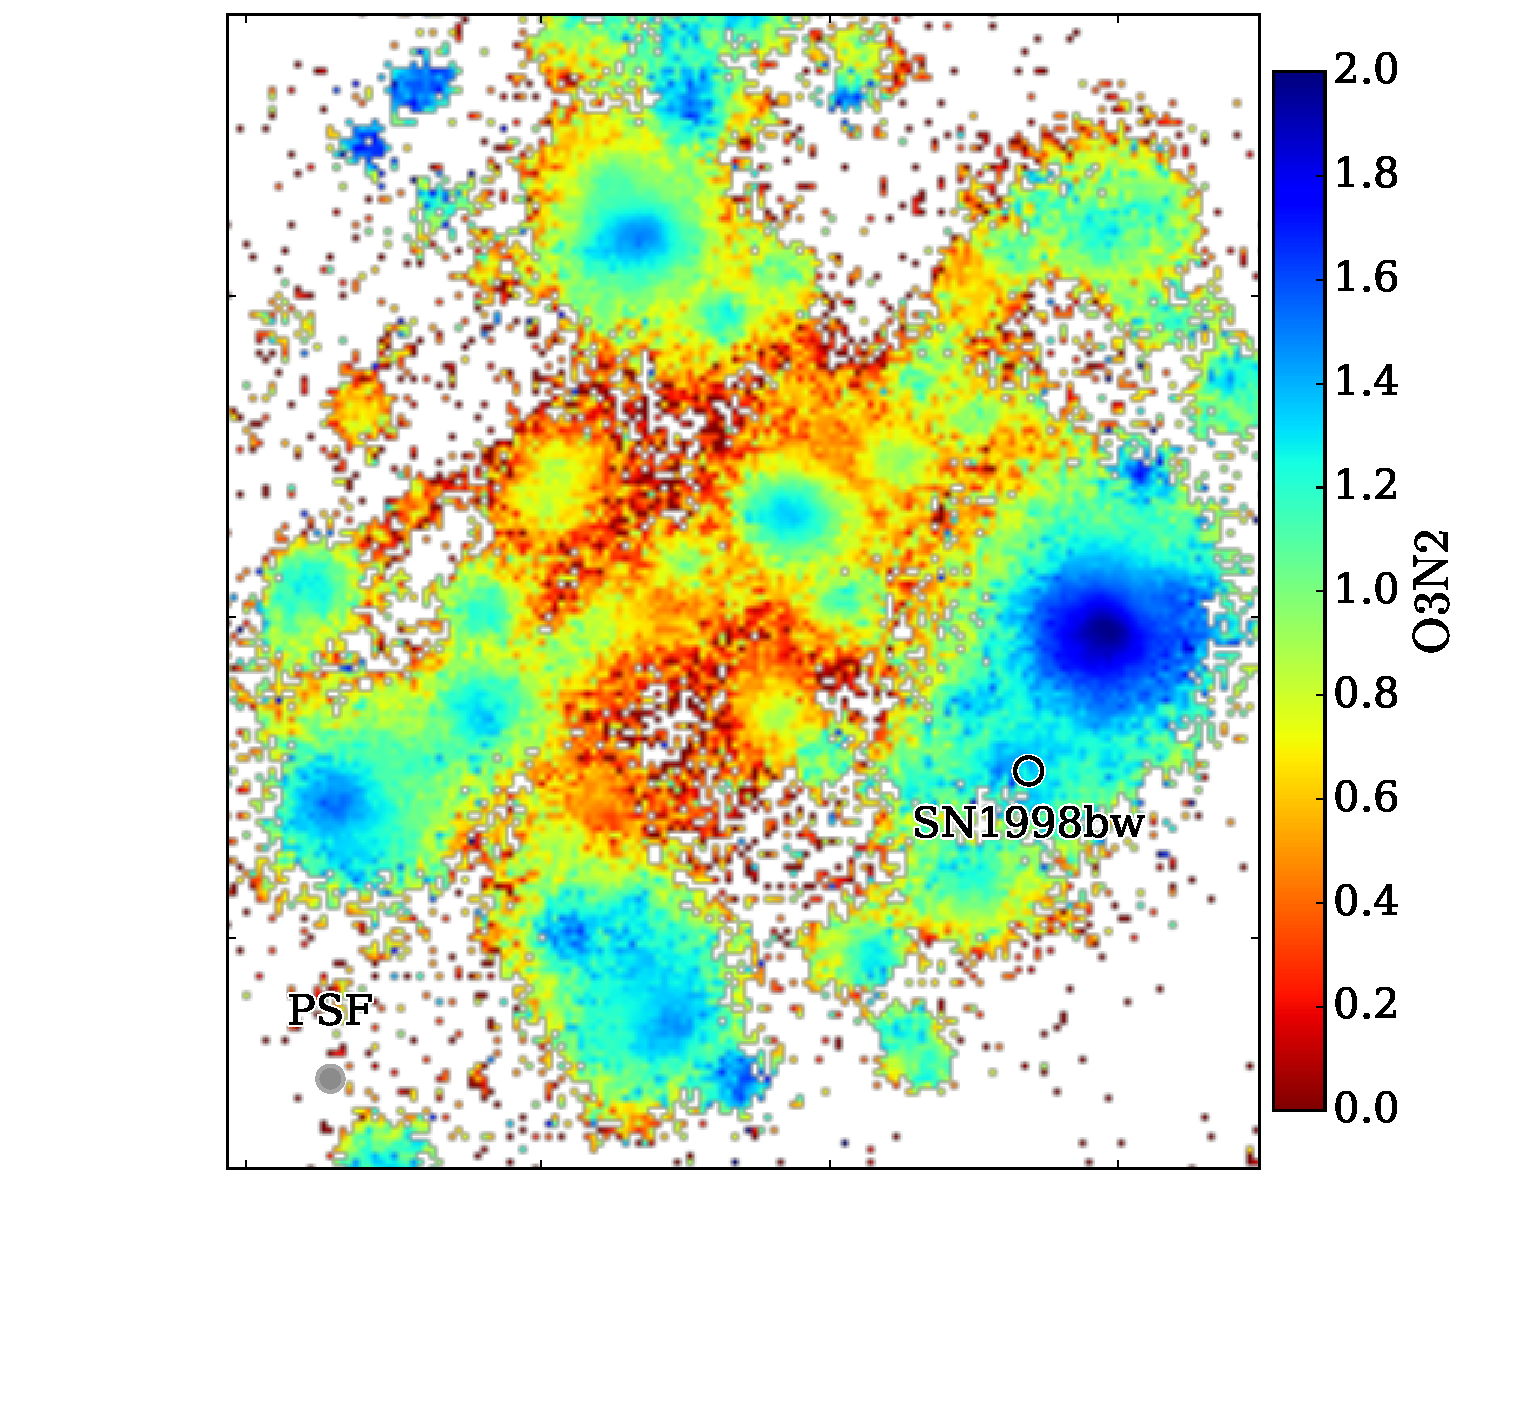
\includegraphics[width=0.999\linewidth]{Figs/MUSE_SN1998bw_O3N2.pdf}
\end{subfigure}
\begin{subfigure}{.24\textwidth}
  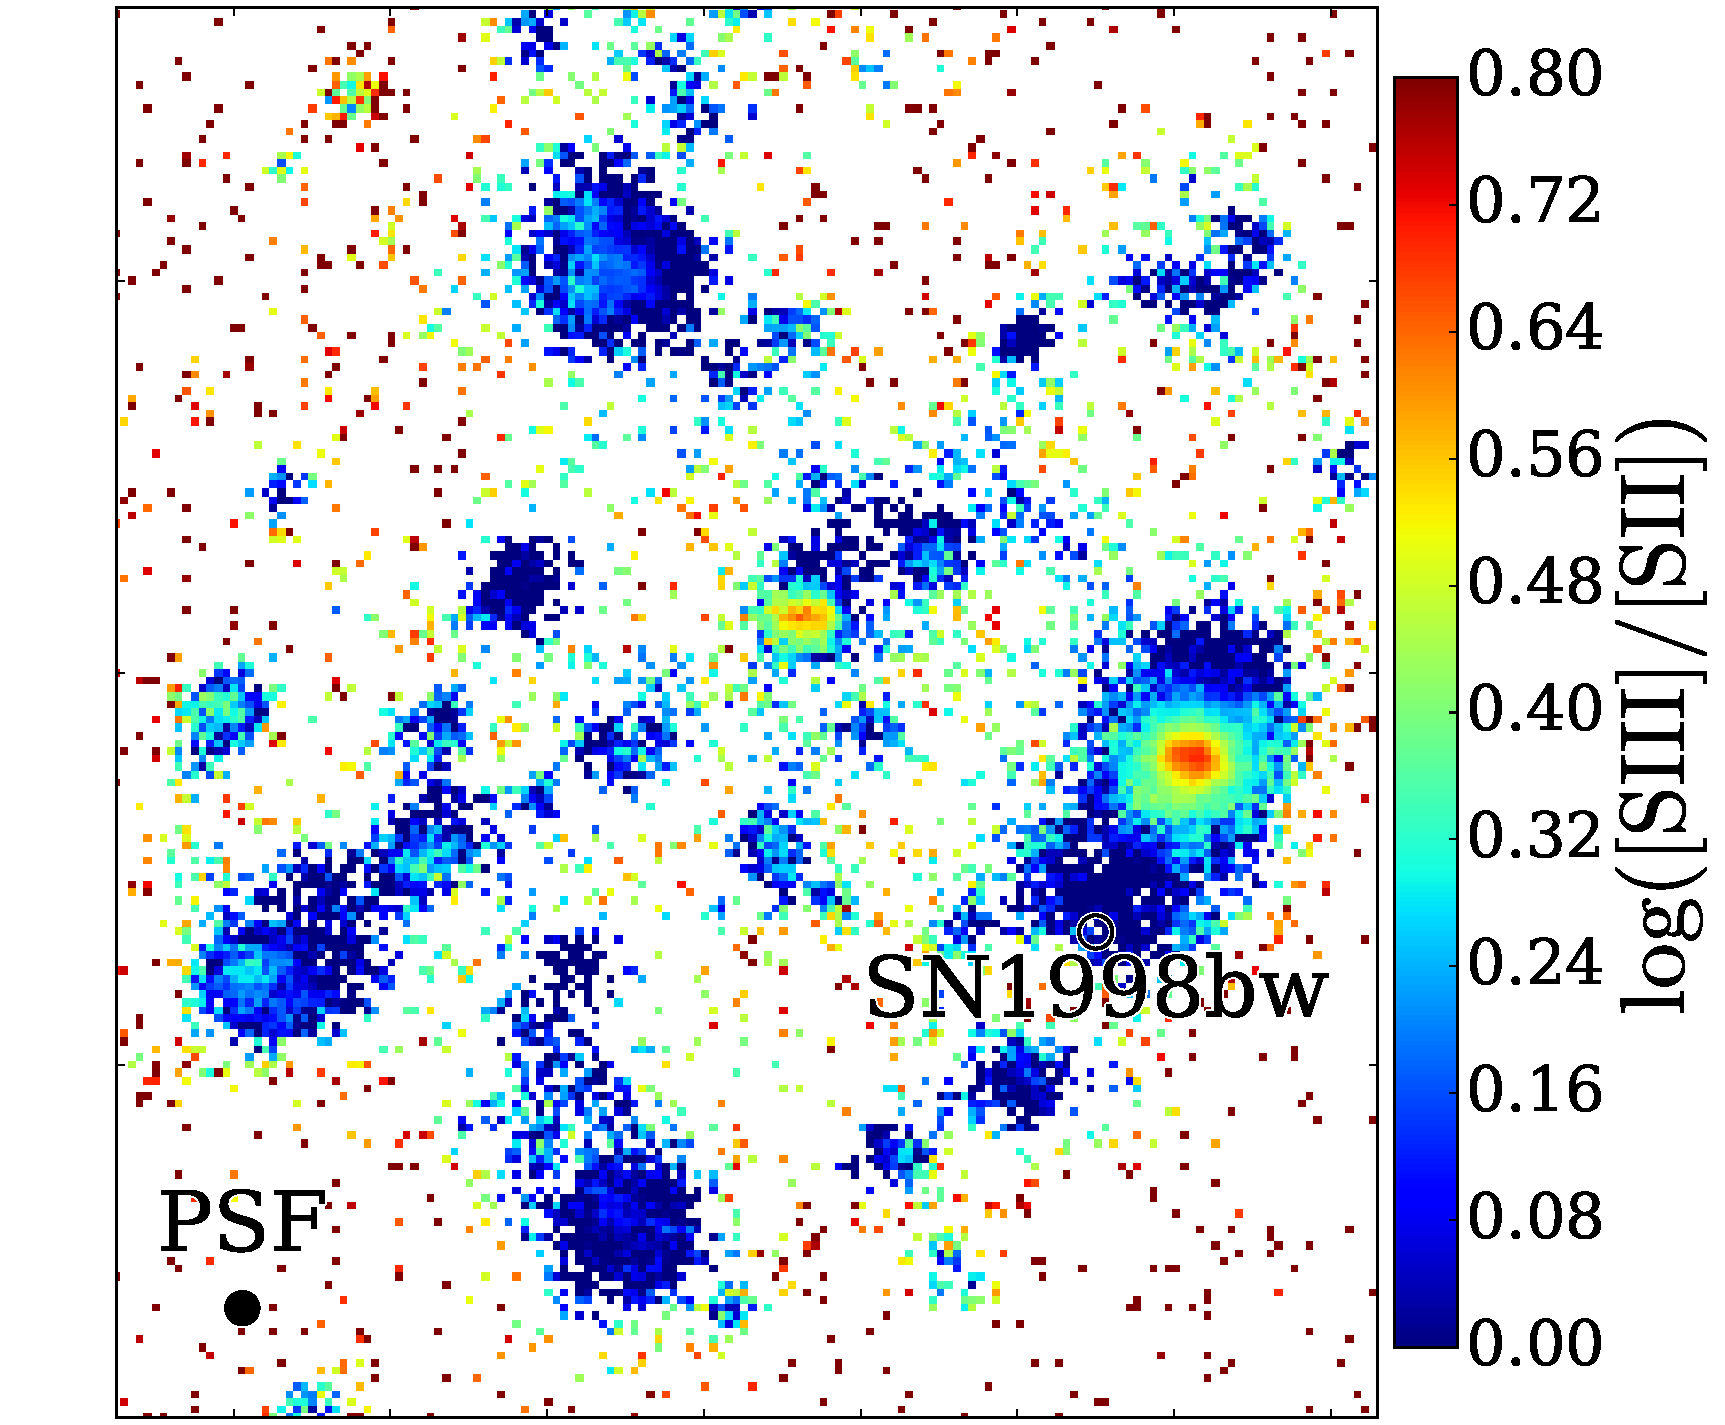
\includegraphics[width=0.999\linewidth]{Figs/MUSE_SN1998bw_S3S2.pdf}
\end{subfigure}
\caption{Face-to-face comparison between the maps of O3N2, often used for abundance determinations and \siii/\sii, a tracer of the ionization state of the hot gas. Only spaxels with SNR > 3 are shown. Image dimensions are similar to Figure~\ref{fig:ebv}.}
\label{fig:s3s2}
\end{figure}

Our MUSE data is of sufficient depth and quality to test how strongly O3N2 is affected by ionization empirically through the ratio of \siii\,(IP=23.3~eV) to \sii\,(IP=10.3~eV), widely considered as one of the best tracers of the ionization parameter \citep{1991MNRAS.253..245D} as it shows in contrast to \oiii/\oii\,only very little dependence on abundance itself \citep{2002ApJS..142...35K, 2011MNRAS.415.3616D}. As MUSE does not cover the wavelength range of \siii($\lambda$9532), we use a theoretical value of $\siii(\lambda9532)=2.44\siii(\lambda9069)$ \citep{1982MNRAS.199.1025M}. The resulting map is shown in Figure~\ref{fig:s3s2} and clearly highlights the \hii~region centers standing out with the largest values of \siii, and thus ionization parameter. %Particular remarkable is the WR-region 800~pc to the North-West of the SN position with $\log($\siii/\sii$)\sim0.8$.

This adds further support to our initial observations of Figure~\ref{fig:o3n2}, and attributes the radial symmetric structure of individual \hii-regions in the O3N2 and N2 maps to an increase of the ionization parameter towards the center of \hii~regions and not chemical inhomogenities. Simple O3N2, or N2-based diagnostic are thus inadequate to produce accurate maps of oxygen abundance at the level of detail of our MUSE data.

\subsubsection{Metallicity maps}
\label{sec:mapoh}

\begin{figure}
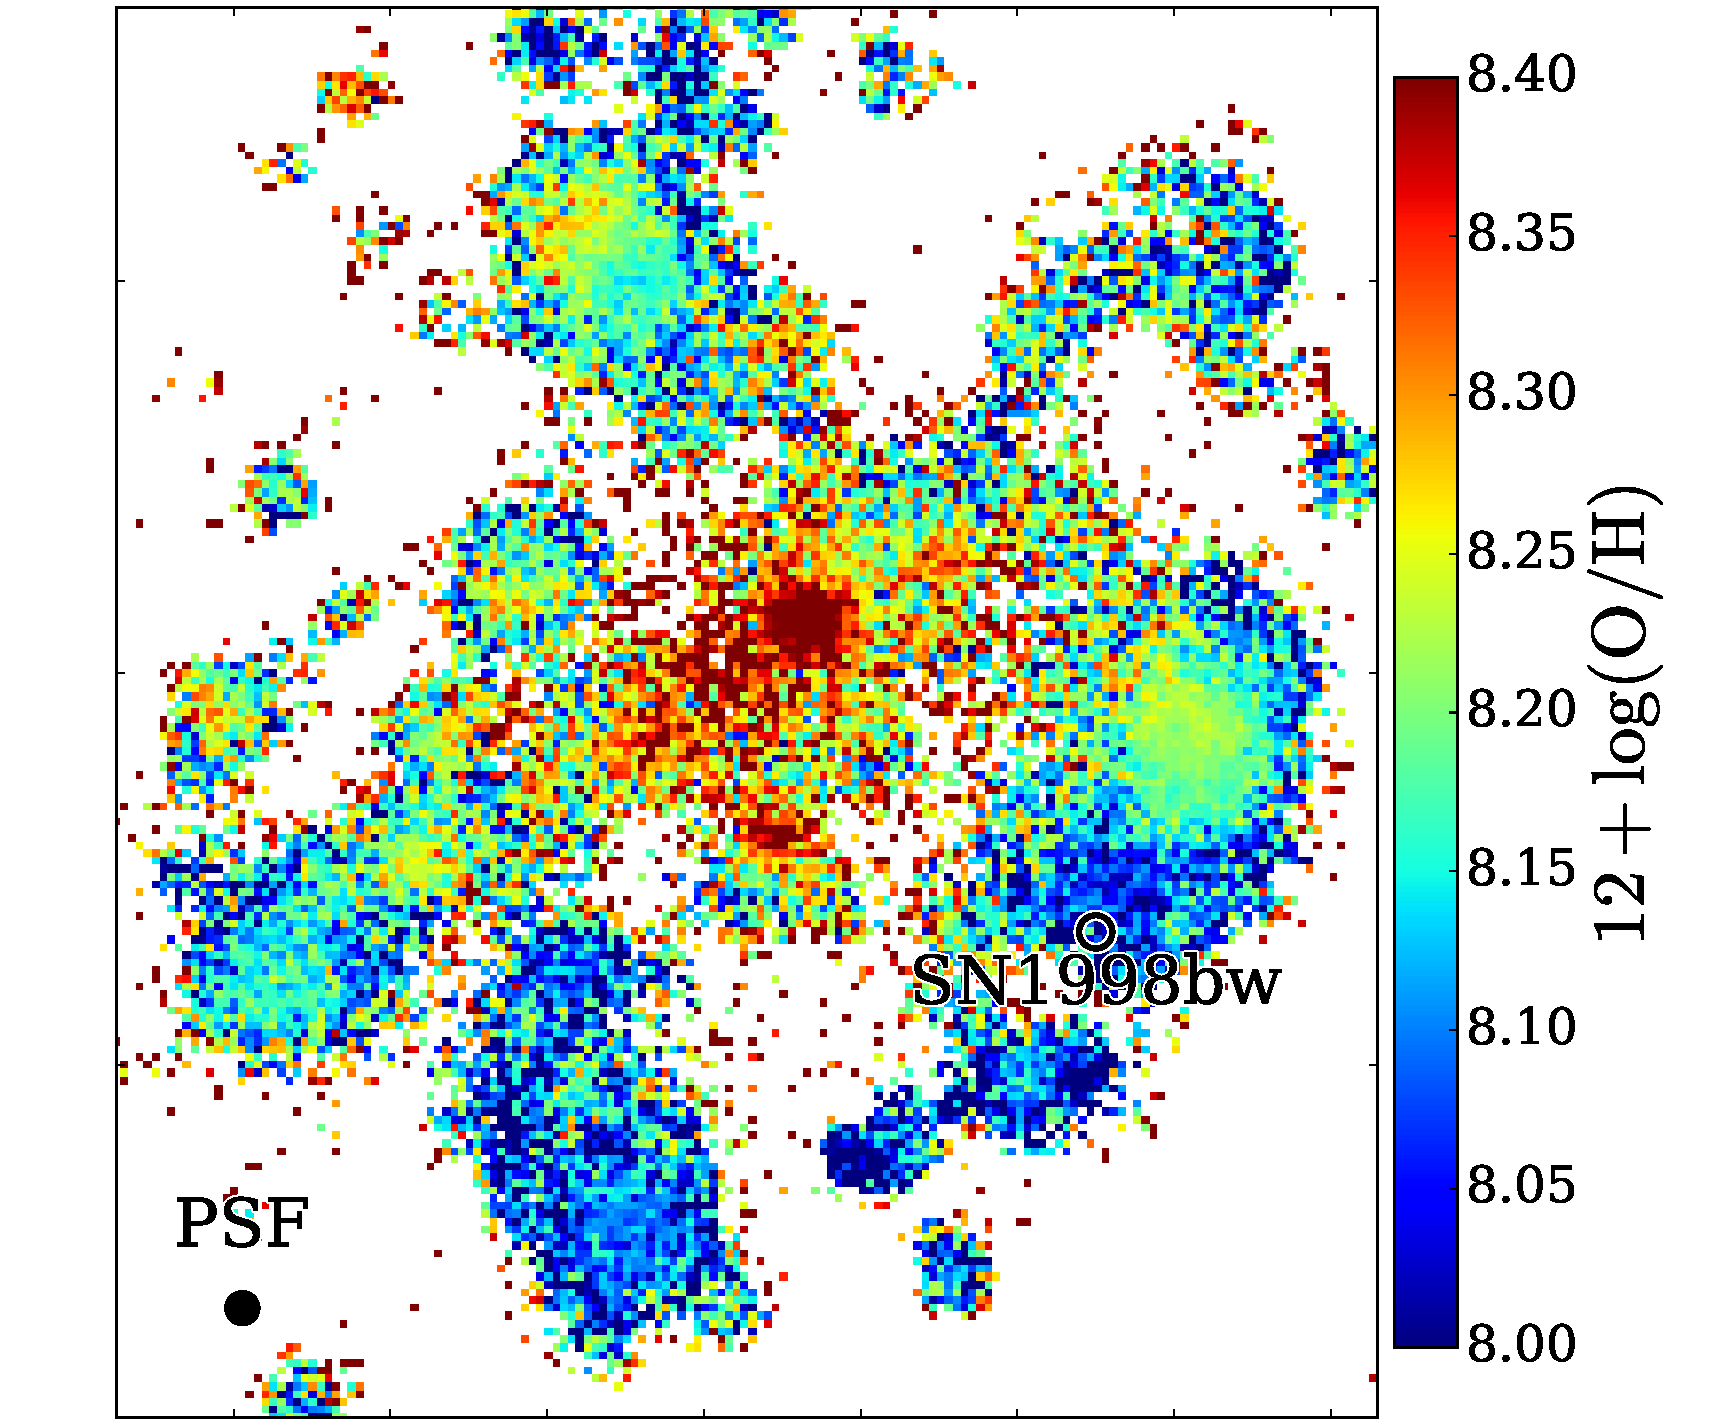
\includegraphics[angle=0, width=0.99\columnwidth]{Figs/MUSE_SN1998bw_OH.pdf}
\caption{Map of \oh\, as obtained through the \sii\, and \nii\, based calibration of \citet{2016Ap&SS.361...61D}. Only spaxels with SNR > 3 are shown. Image dimensions are 34" by 38", or 6.1~kpc by 6.8~kpc, similar to Figure~\ref{fig:ebv}. The circle denoting the position of SN\,1998bw has a radius of 180 pc}
\label{fig:s2}
\end{figure}

After rejecting empirical methods using O3N2 or N2 as reliable metallicity tracer due to their ionization dependence, we turn to diagnostics based on photo-ionization models. Unfortunately, most of the previous strong-line methods rely in one way or another on \oii\,\citep{2002ApJS..142...35K}, which is not available to us here. Also \siii/\sii\, is a good ionization tracer, but \siii\,is relatively faint and not detected in most of our spaxels (see Figure~\ref{fig:s3s2}). A recently published method based on photo-ionization modeling \citep{2016Ap&SS.361...61D} seems to perfectly fit to our data. It relies solely on \ha, \nii, and \sii, which are all strong and well within the wavelength range of MUSE. The method is introduced as "effectively independent of both ionization parameter and ISM pressure" \citep{2016Ap&SS.361...61D}, and Figure~\ref{fig:s2} displays the respective map of \oh\, in regions where the necessary lines are detected at sufficient SNR.

Clearly, the strong abundance gradient over individual \hii-regions as would have been deduced from O3N2, is not observed in this diagnostic. Instead, the oxygen abundance map displays a relatively smooth behavior with a decreasing overall metallicity from the center of the galaxy towards the outside (see also Section \ref{sec:metgrad}). The oxygen abundance at the spaxel that is closest to the SN position is \oh=8.00 or 0.20\,Z$_{\odot}$. The immediate environment is consistent with this value and relatively homogeneous: the spaxels within a radius of 70 pc to the SN position have \oh$=8.06\pm 0.06$. The WR region displays a somewhat higher metallicities with the oxygen abundances of at the peak of the \ha\,emission yielding \oh$=8.21\pm 0.03$ or $0.33\pm0.03\,$Z$_{\odot}$.

It is of course reasonable to ask now whether the new \citet{2016Ap&SS.361...61D} diagnostic provides more reliable constraints on oxygen abundance than previous methods, in particular given the significant differences when compared to abundances derived in previous works. In addition, for low-mass galaxies as is the case here, this diagnostic seems to return lower oxygen abundances than previous methods \citep{2016ApJ...823L..24K}. To elaborate further on the \sii-based diagnostic, we reproduce Equation 1 and 2 from \citet{2016Ap&SS.361...61D}

\begin{equation}
12+\log(\mathrm{O/H}) = 8.77 + \log([\ion{N}{ii}]/[\ion{S}{ii}]) + 0.264\log([\ion{N}{ii}]/\mathrm{H}\alpha)
\end{equation}

with \nii\, being the flux in the \nii($\lambda6484$) line, and \sii\, the flux in the \sii($\lambda\lambda6717,6731$) doublet. The primary observable is thus the nitrogen to sulfur ratio, which is a tracer of the nitrogen to oxygen ratio\footnote{Sulfur and oxygen are both $\alpha$-process elements produced in massive stars, and observed to track each other well in different environments \citep[see e.g., Figure 6 in][]{2006A&A...448..955I}.}. Because nitrogen is also produced in intermediate mass stars, N/O starts to depend on \oh\,above \oh$\sim 7.6$ \citep[e.g.][]{1999ApJ...511..639I, 2013A&A...549A..25P}, and as expected, a N/O map via \citet{2010ApJ...715L.128A} is very similar to the map of oxygen abundance in the respective strong line diagnostic. 

The map of oxygen abundance then fundamentally relies on the N/O-to-O/H, calibration, and it is in principle not impossible that there are internal variations in N/O at a given \oh, or differences between the host of SN\,1998bw to the calibration sample. For example infall of primordial gas would decrease \oh, but leave N/O unaffected \citep{2016ApJ...823L..24K}. Another point of concern would be an anomalously high N/O ratio for the SN region as claimed in \citet{2006A&A...454..103H}. However, both of these effects would lead us to over predict the actual oxygen abundance in the SN region, whereas we observe some of the lowest values here. Also the calibration sample for N/O-to-O/H in the metallicity range of interest is based on low-metallicity blue compact dwarf galaxies \citep{1999ApJ...511..639I}, not dissimilar in physical properties to our galaxies. %An illustrative comparison is also the host of the SLSN PTF12dam \citep{2015MNRAS.451L..65T}, which shows similar EW

\subsubsection{Temperature-based metallicities}

\begin{figure}
\begin{subfigure}{.24\textwidth}
  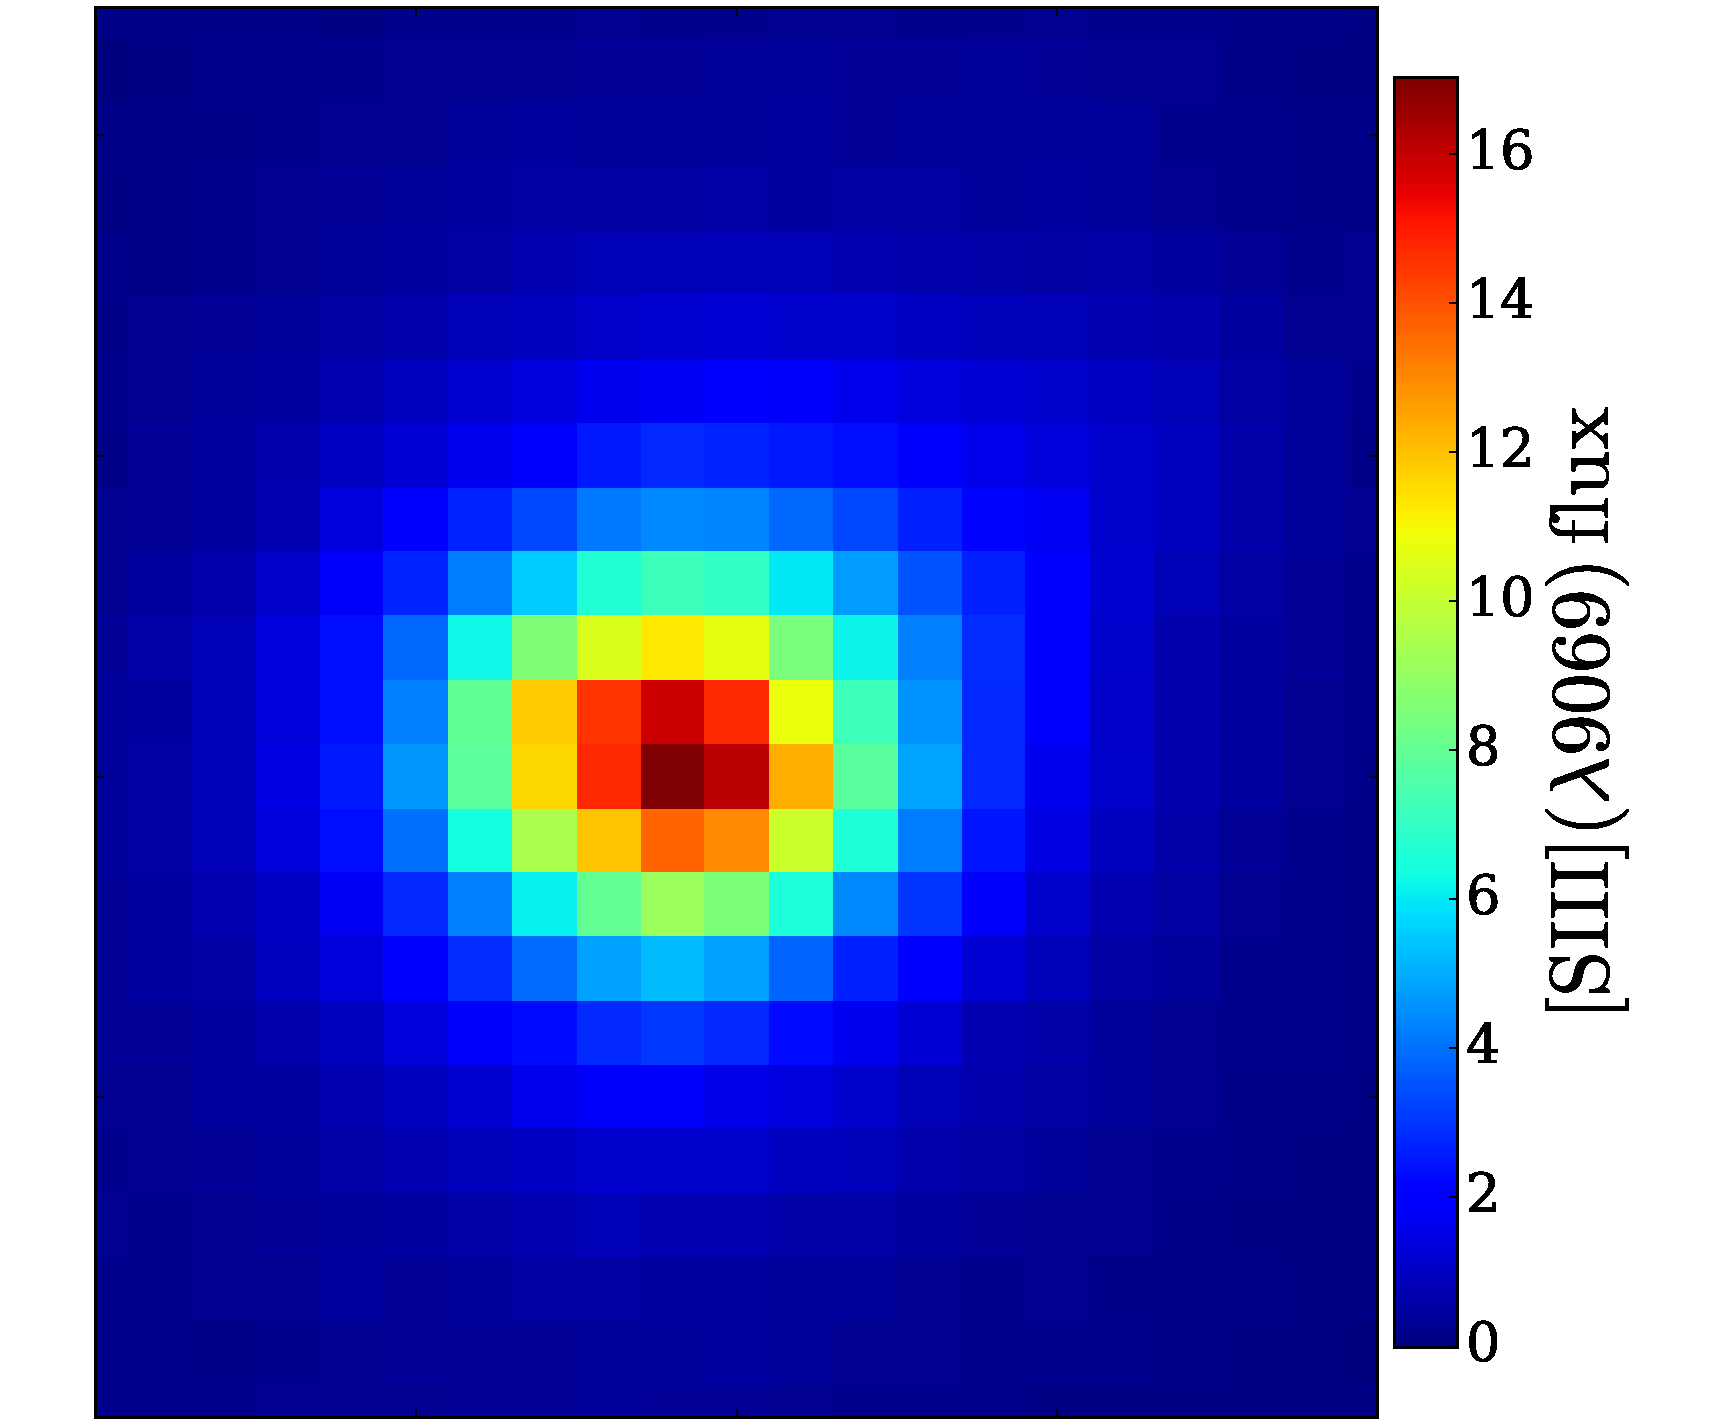
\includegraphics[width=0.999\linewidth]{Figs/MUSE_SN1998bw_SIIIzoom.pdf}
\end{subfigure}
\begin{subfigure}{.24\textwidth}
  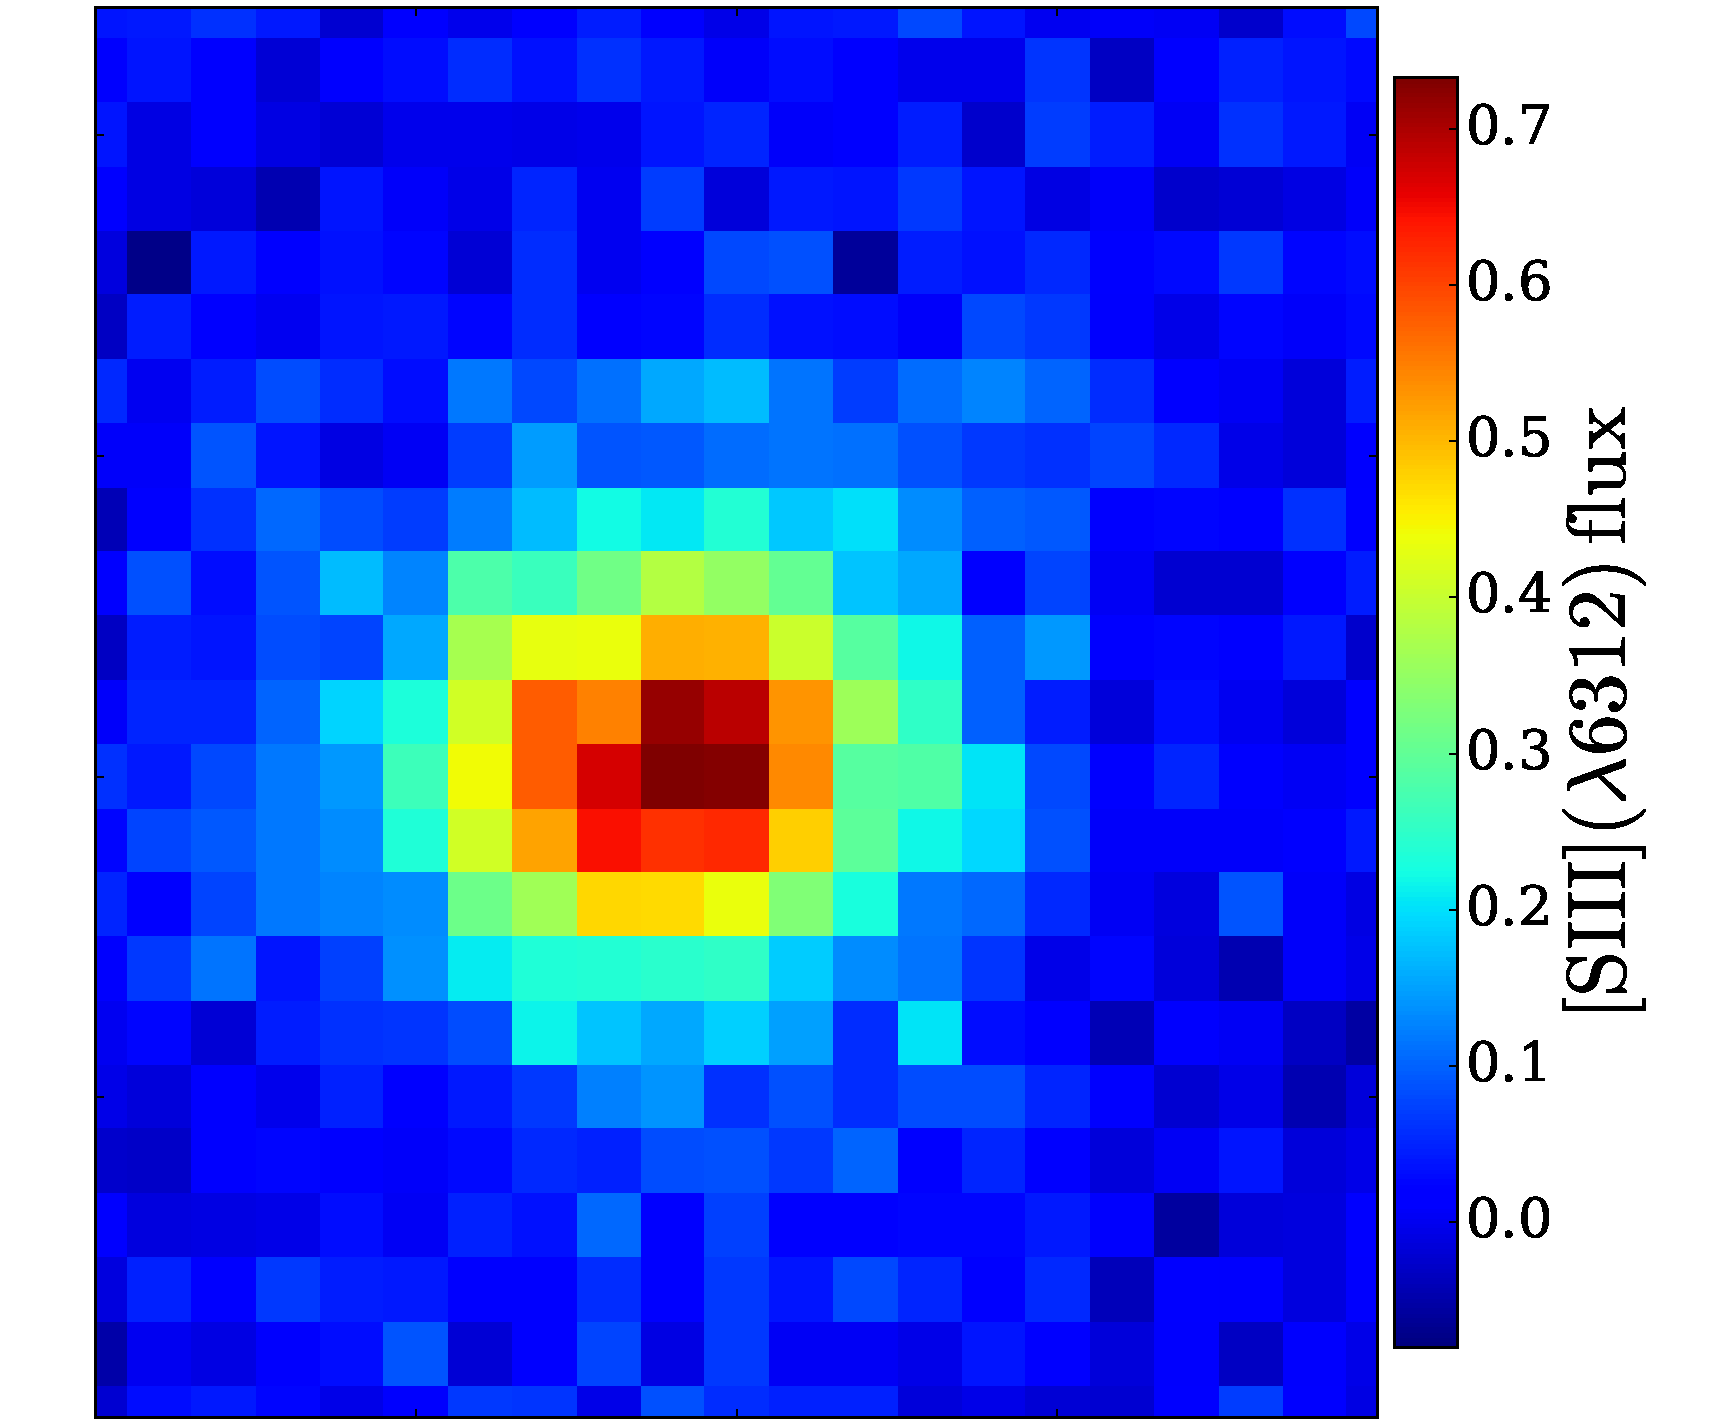
\includegraphics[width=0.999\linewidth]{Figs/MUSE_SN1998bw_SIIIauzoom.pdf}
\end{subfigure}
\begin{subfigure}{.24\textwidth}
  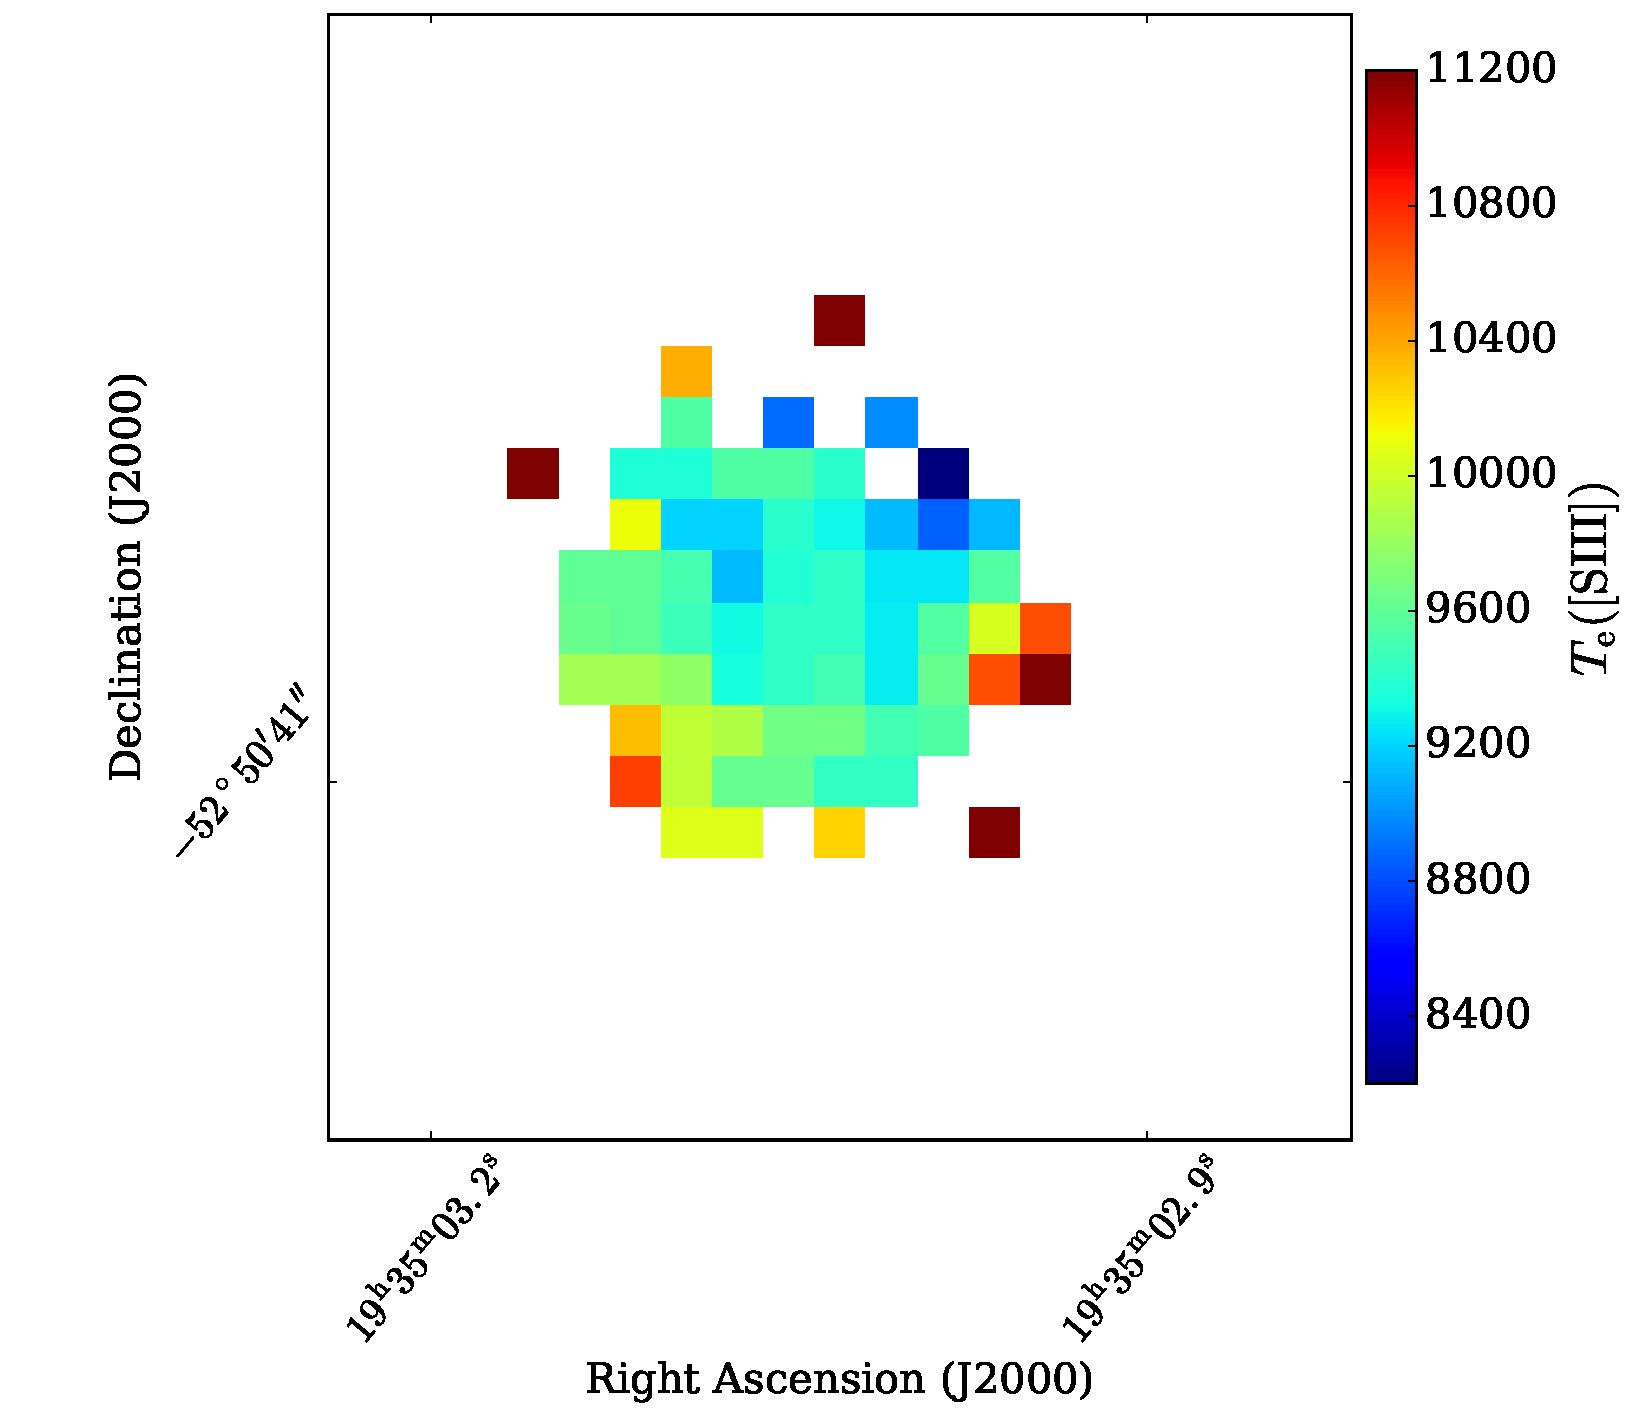
\includegraphics[width=0.999\linewidth]{Figs/MUSE_SN1998bw_T.pdf}
\end{subfigure}
\begin{subfigure}{.24\textwidth}
  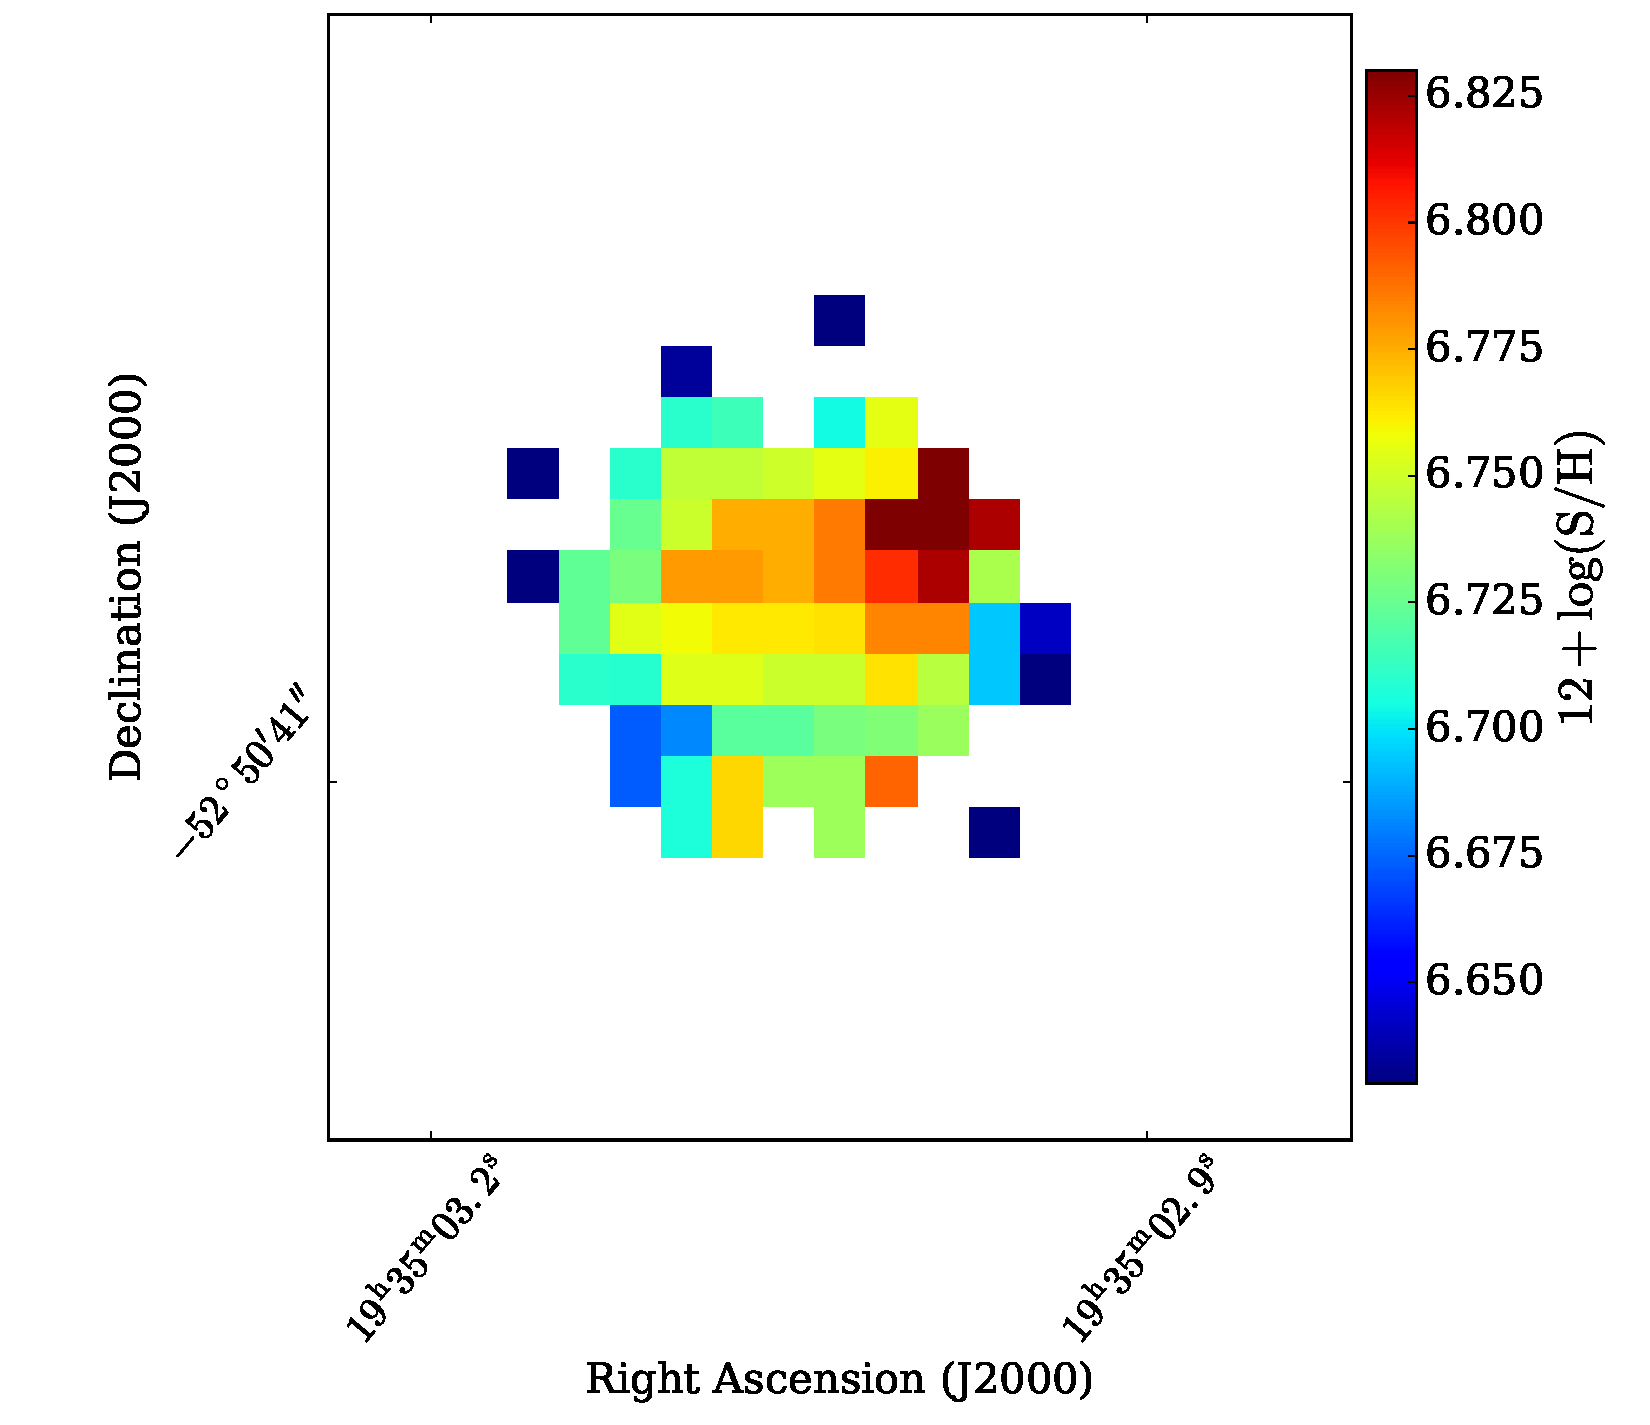
\includegraphics[width=0.999\linewidth]{Figs/MUSE_SN1998bw_SHTzoom.pdf}
\end{subfigure}
\caption{Zoom-in to the WR region for temperature estimation. top-left: nebular \siii($\lambda9069$), top-right: auroral \siii($\lambda6312$), bottom-left: \siii\, electron temperatures, bottom-right $12+\log(\mathrm{S/H}$ as derived from the electron temperature, \sii($\lambda\lambda6717,6731$). The relative abundance of oxygen and sulfur in the sun [O/S] is 1.57 \citep{2009ARA&A..47..481A}, so the plotted $12+\log(\mathrm{S/H})$ scale corresponds to \oh = 8.2 to 8.4. All panels are approximately 6" by 6", or 1 by 1 kpc. One MUSE spaxel corresponds to 35~pc.}
\label{fig:temp}
\end{figure}

Given the significant discrepancies that exist between our and previous measurements of oxygen abundance for the SN\,1998bw environment, we further seek to corroborate our earlier measurements through temperature-sensitive lines. Unfortunately, \oiii($\lambda$4363) is not covered by the MUSE wavelength response, and the other, fainter temperature-sensitive lines are too faint to be detected in most of the individual spaxels. However, we clearly detect both \siii($\lambda$6312) in the WR region (Figure~\ref{fig:temp}), and in a integrated spectrum from spaxels within a radius of 0\farc{8} around the SN position. 

%\begin{figure}
%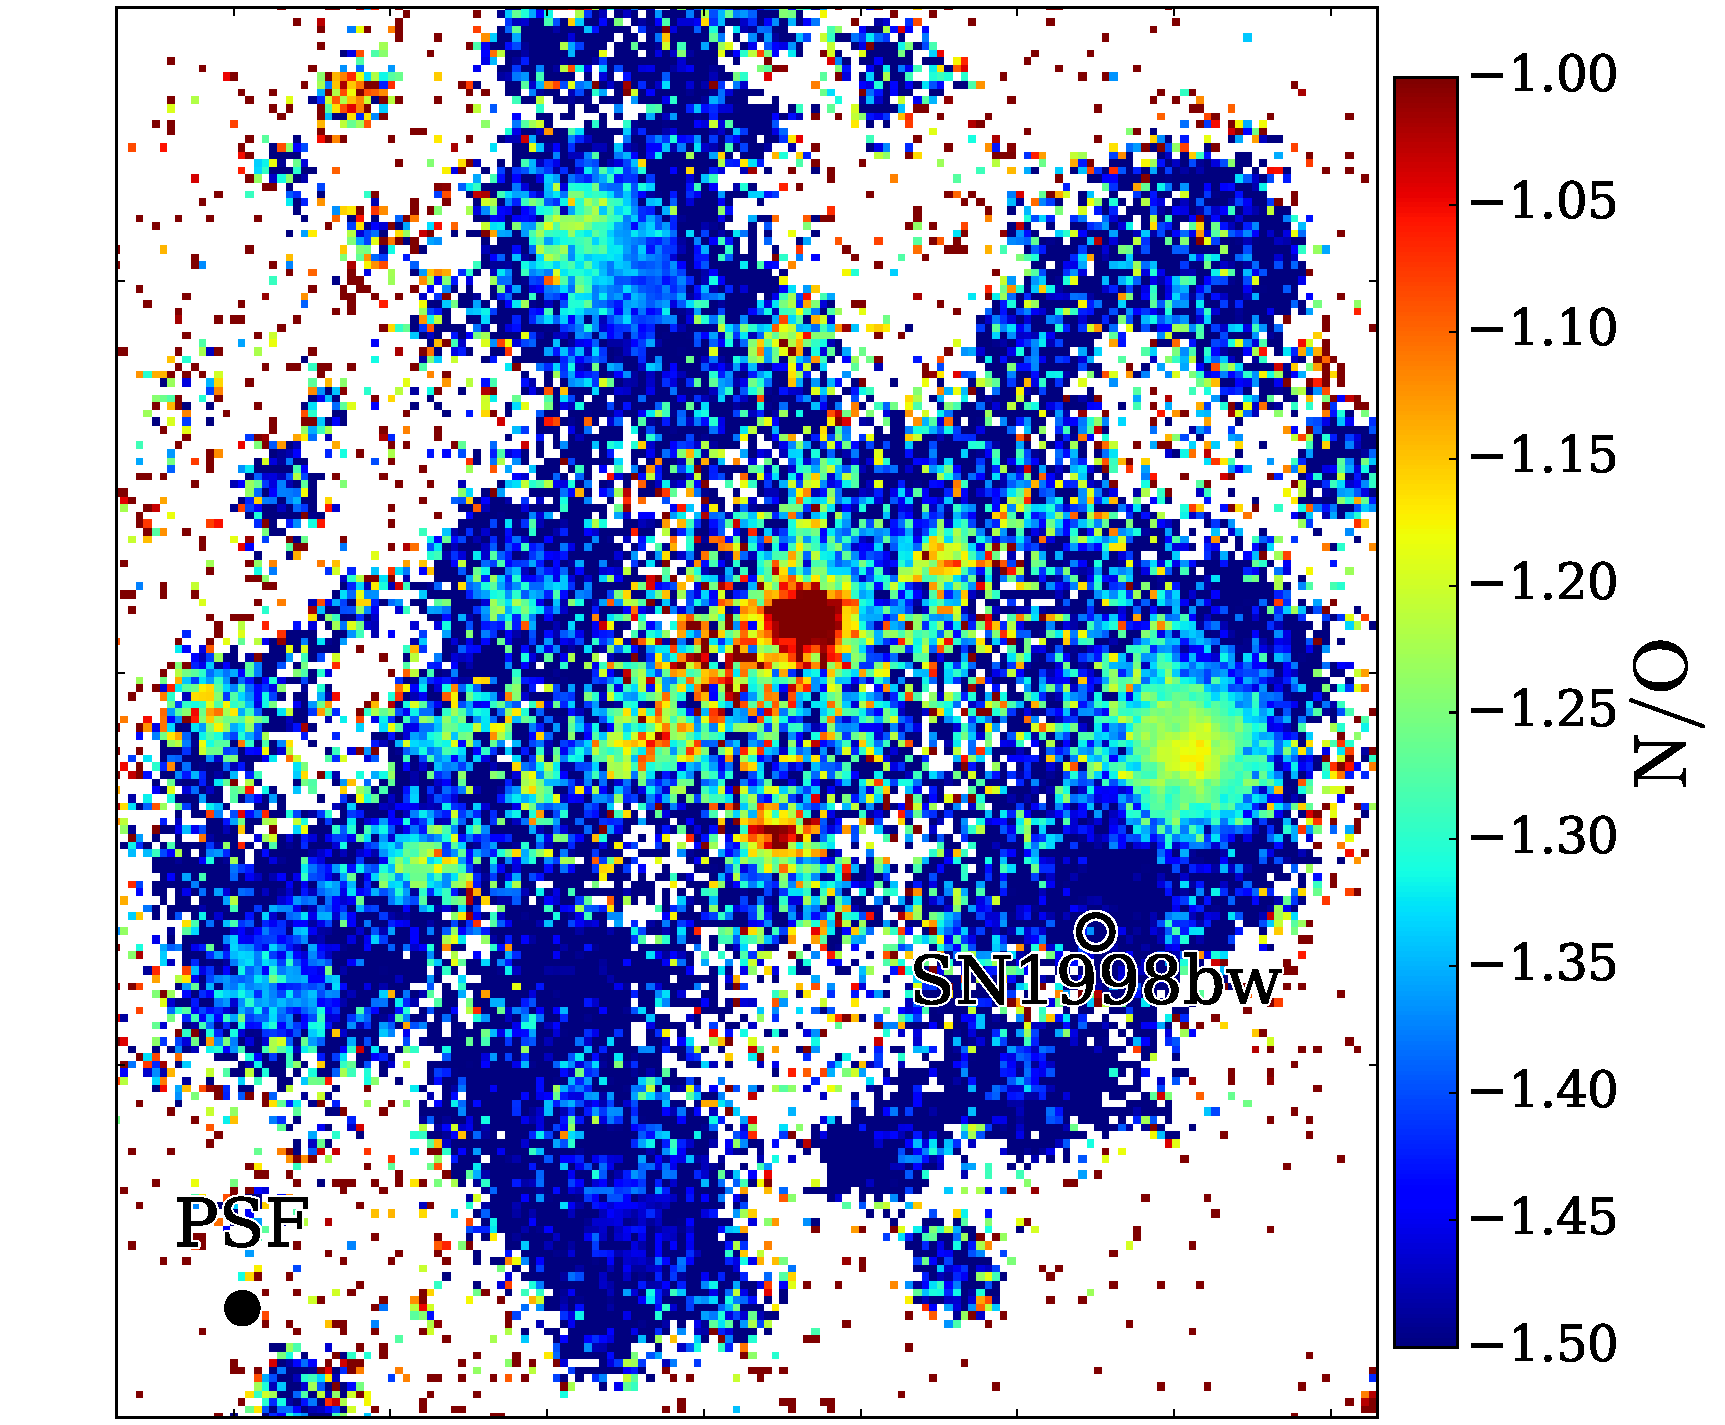
\includegraphics[angle=0, width=0.99\columnwidth]{Figs/MUSE_SN1998bw_NO.pdf}
%\caption{Map of N/O. Image dimensions are similar to Figure~\ref{fig:ebv}}
%\label{fig:no}
%\end{figure}

Using most recent atomic data and following \citet{2013ApJS..207...21N}, we derive an electron temperature from \siii\, in the central part of the WR-region of around $T(\mathrm{e}_{\siii}=(0.94\pm0.04)\cdot10^{4}$~K. Figure~\ref{fig:temp} contains maps of the crucial emission lines (nebular \siii($\lambda9069$, and auroral \siii($\lambda$6312)), the resulting temperatures as well as sulfur abundances. These values correspond to somewhat larger temperatures of \oiii~of around $T_{\oiii} \sim 1.07\cdot10^{4}$~K \citep{2006A&A...448..955I, 2012A&A...547A..29B}. The flux in the doublets of \oii($\lambda\lambda$7320,7330) and \oiii($\lambda\lambda$4959,5007) then yields central abundances of the WR region around \oh $\sim 8.3$. 

Similar values are obtained when using solar abundances to convert the sulfur to an oxygen abundance. These are somewhat (0.10-0.15~dex.) higher than implied by the strong line diagnostic from Section \ref{sec:mapoh}, but critically depend on the sulfur-to-oxygen temperature conversion or assumed abundance. They are thus subject to some systematic uncertainties. However, it is clear that the strong structure in O3N2 or N2 over the \hii-region are not observed in electron temperatures.

Emission-lines in the SN region are substantially fainter, and only detected in a stacked spectrum extracted from 3x3 spaxels around the SN position. In a similar way as above, we constrain the temperature in the SN region through \siii\, to $T_{\mathrm{e}}(\siii)=(1.24\pm0.18)\cdot10^{4}$~K, slightly higher than in the WR-region, but with large uncertainties. 

To better constrain $T_{\mathrm{e}}(\oiii)$, we re-reduce the VLT/FORS2 long-slit spectroscopy data of \citet{2006A&A...454..103H} as it covers both WR-region and SN position and extends below $4000\,\AA$. Using the well-detected \oiii($\lambda$4363) line, we measure temperatures of $T_{\mathrm{e}}(\oiii)=(1.05\pm0.05)\cdot 10^{4}$~K and $T_{\mathrm{e}}(\oiii)=(1.42\pm0.18)\cdot10^{4}$~K for the WR and SN region, respectively. These values from the FORS data are broadly consistent with the estimates from MUSE through \siii($\lambda$6312), and yield oxygen abundances of \oh=$8.39\pm0.07$ and $8.01\pm0.10$ for WR and SN region. 

The WR thus does not exhibit the lowest metallicity within its host as claimed previously \citep{2008A&A...490...45C}. This observation was rather an artifact from the dependence of the O3N2 strong line diagnostic on ionization.

Our relatively low oxygen abundances at the location of SN (\oh$\sim8.1$) and WR-region (\oh$\sim8.3$), as well as galaxy integrated values ($\sim8.2$) correspond to 0.2 to 0.4 times the solar value, and thus explains many of the long-wavelength properties of ESO184-G82 as typical for metal poor dwarf galaxies without invoking a deficiency in molecular gas \citep{2016arXiv160901742M}.

%\section{Discussion and Implications}

\subsection{Metallicity gradients}
\label{sec:metgrad}

\begin{figure}
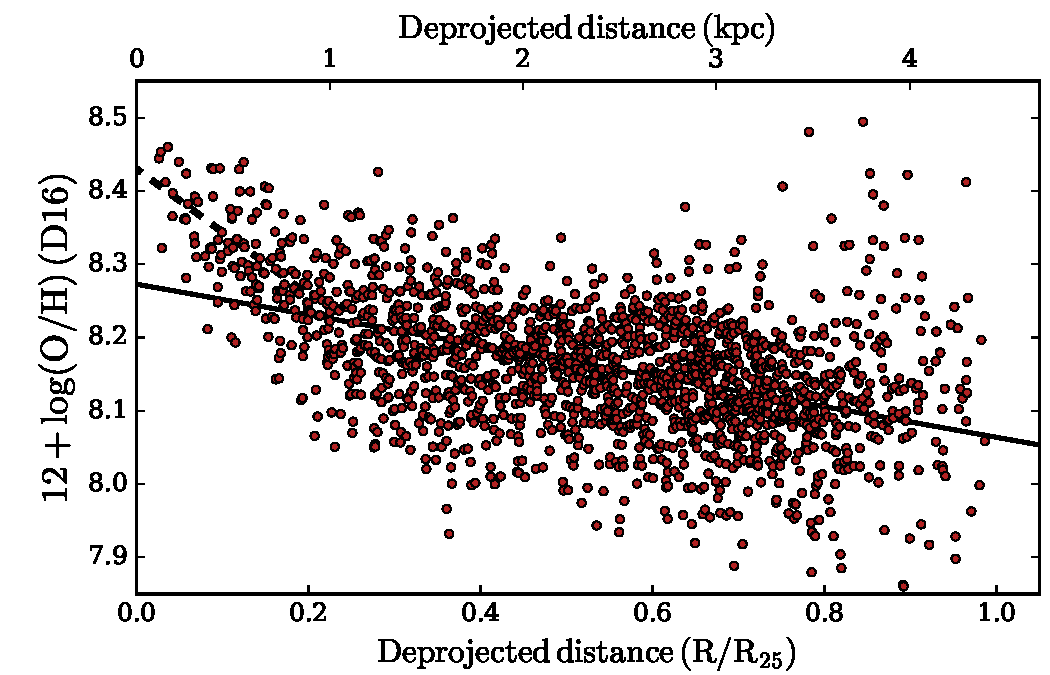
\includegraphics[angle=0, width=0.99\columnwidth]{Figs/MUSE_SN1998bw_metgrad.pdf}
\caption{Metallicity gradient.}
\label{fig:metgrad}
\end{figure}

The metallicity of galaxies is often observed to decrease with the distance from their centers \citep[e.g.,][]{1994ApJ...420...87Z, 2014A&A...563A..49S}, also observed in the hosts of SNe \citep{2016A&A...591A..48G}. These gradients are important to understand for spatially-unresolved studies at high redshift, where positional offsets can be measured, but abundances are only derived in a galaxy integrated manner. From Figure~\ref{fig:s2}, its immediately clear that we are observing a similar effect. The center of ESO184-G82 is significantly more chemically-enriched than the outer regions. 

Figure~\ref{fig:s2} shows the oxygen abundance of individual regions as a function of their distance to the center. Each data point represents the median oxygen abundance in a region of 3 by 3 spaxels each detected at a S/N of at least 5. The galaxy center is measured as the luminosity-weighted center of the $R$-band light at RA(J2000)=19:35:04.40, Decl.(J2000)=-52:50:38.0, around 3" South-East of the \hii-region with the highest metallicity (Figure~\ref{fig:s2}) and the second highest ionization (Figure~\ref{fig:s3s2}). To obtain Figure~\ref{fig:s2}, we assumed an inclination of ESO184-G82 of $50^{\circ}$ \citep{2008A&A...490...45C, 2015MNRAS.454L..51A}, as well as a position angle of $145^{\circ}$ \citep{1989spce.book.....L}. 

Using a linear regression on the data of Figure~\ref{fig:metgrad}, the metallicity gradient is best-fit with a slope of $0.25\pm0.01$~dex/$R_{25}$ in relative, or 0.056~dex/kpc in physical scales, well in the range that was previously measured for galaxies of comparable stellar mass \citep{2015MNRAS.448.2030H}. Here, $R_{25}$ is the radius at the $B=25\,\mathrm{mag}\,\mathrm{arcsec}^2$ isophotal. O3N2-based diagnostics return slightly steeper, but within errors generally compatible values. The linear fit to the oxygen abundance data is a reasonable description of the data, except for the very center below a deprojected distance of 1~kpc, where the metallicity is seen to decrease more steeply. Limiting the fit range to data below 1~kpc, we derive the slope in the central kpc to $0.85\pm0.10$~dex/$R_{25}$ or 0.18 dex/kpc (see dashed line in Figure~\ref{fig:metgrad}). 

A comparison between this metallicity gradient to the typical values of (projected) GRB distances from the galaxy centers of 1.3~kpc \citep{2016ApJ...817..144B} does not provide strong reason to suggest that the average measurement of GRB host metallicities from spatially-unresolved data is significantly skewed when compared to the GRB site metallicity. There is however a non-negligible fraction of GRBs at substantial distances to their hosts (10\% at $>3$~kpc) where metallicity gradients might lead to overestimates on the GRB site abundance from unresolved spectra.

Figure~\ref{fig:metgrad} also illustrates the typical spread of oxygen abundances at a given galactic radius. With an root-mean-square (RMS) spread below 0.1~dex below $R_{25}$, and we find no evidence for extremely ($Z < 0.1 Z_\odot$) gas-poor regions at the spatial scales probed by our observation (100 pc). 

\subsection{ESO184-G82 if seen at high redshift}

%\begin{figure}
%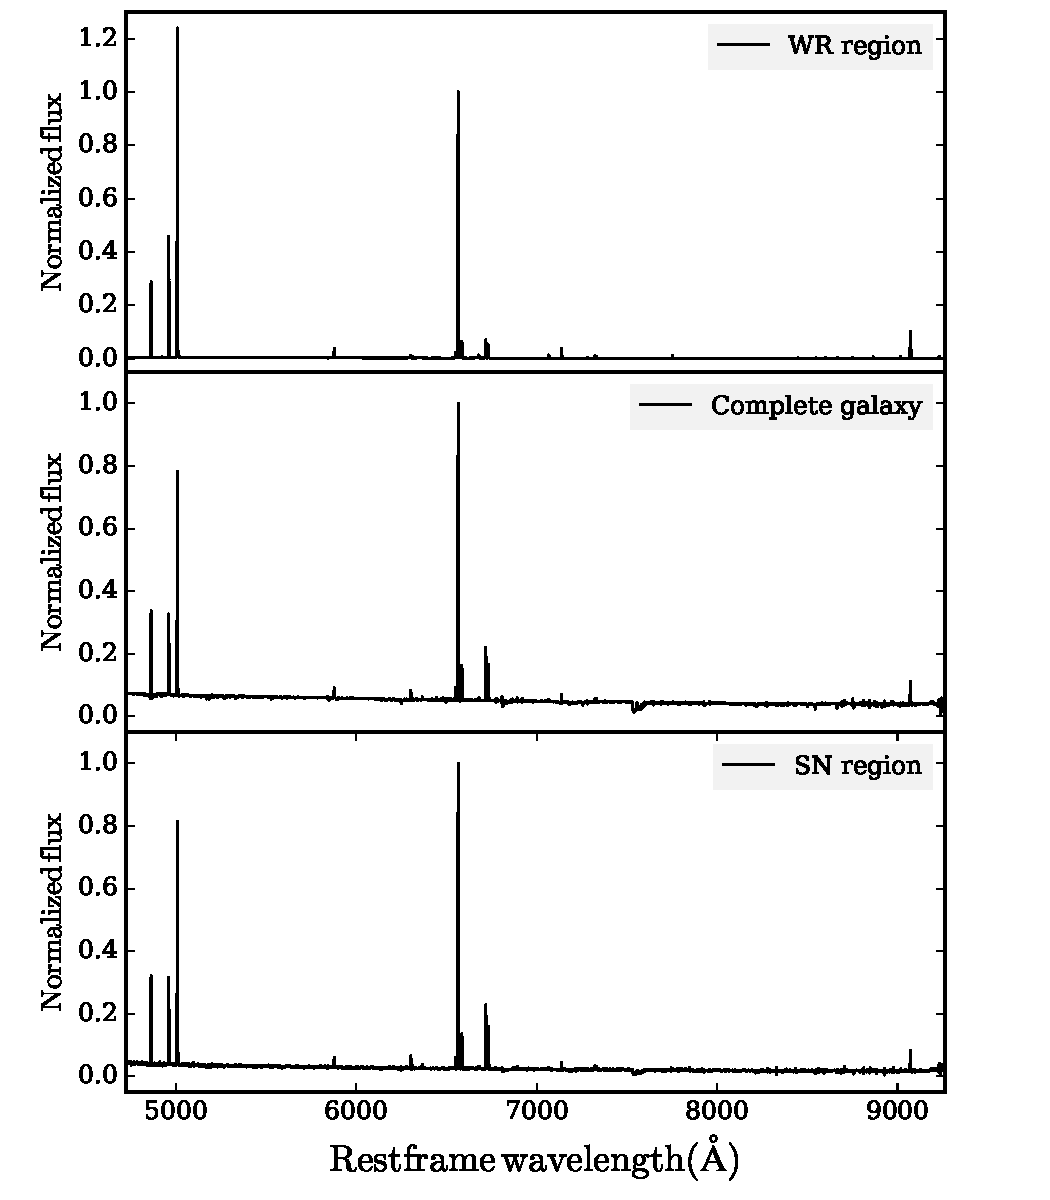
\includegraphics[angle=0, width=0.99\columnwidth]{Figs/SN1998bw_specs.pdf}
%\caption{Metallicity gradient}
%\label{fig:specs}
%\end{figure}

GRB\,980425/SN\,1998bw is the closest GRB detected in two decades, and an exceptional opportunity to measure the physical parameters of its host within high precision and high spatial resolution. Typically, information on environments of GRBs or similar kind of transients  at higher redshift is obtained only in a galaxy-integrated fashion\citep{2015A&A...581A.125K, 2016A&A...590A.129J}, where it is far from obvious whether the measured parameters actually correspond to GRB/SN location properties. We thus seek to compare the GRB explosion site spectrum extracted from the 9 closest spaxels to a galaxy-integrated spectrum as it would appear if it were unresolved and observed through a long-slit. 

First, we compare the total SFR as derived from integrating all spaxels after a reddening correction ($SFR=0.23\pm0.02$\,\Msunyr), to the value what would inferred from the \ha\,flux corrected from the $E_{B-V}=0.07\pm0.01$ derived from the integrated spectrum ($SFR=0.18\pm0.01$\,\Msunyr). Both values nicely agree with FIR, \oi, and \cii\, derived SFRs \citep{2014A&A...562A..70M, 2016arXiv160901742M}, and the narrow-band \ha\, image from \citet{2005NewA...11..103S} once their Salpeter IMF is taken into account. The difference to other \ha\,-derived SFR \citep{2006A&A...454..103H, 2008A&A...490...45C} is entirely due to their overestimated dust correction and a different IMF.

We then derive physical parameters from the spectra of the explosion site, the central part of the Wolf-Rayet region, and the integrated galaxy within a diameter of 50" around its center as summarized in Table~\ref{tab:prop}. There is good agreement between many of the physical properties of the galaxy and the SN site spectrum. Not unexpectedly, resolved measurement of EWs at the SN site are somewhat higher, whereas both dust (by 0.02~mag) and oxygen abundance (by 0.1~dex) are somewhat lower at the SN site than for a galaxy integrated spectrum. ESO184-G82 thus does not provide strong evidence that GRB position spectra are markedly different from galaxy-integrated values. Whether this observation remains valid for a larger sample of GRB hosts remains to be tested of course.

Comparing table~\ref{tab:prop} with Figures~\ref{fig:metgrad} and \ref{fig:s2} also illustrates that the oxygen abundance derived from a galaxy-integrated spectrum is not the central abundance of the galaxy. As the metallicity determination in an unresolved case is a SFR-weighted measurement, it is dominated by \hii-regions primarily located offset from the center as illustrated in Figure~\ref{fig:HaEW}, so it corresponds to a  distance of around $2-3$ kpc from the center. 

\begin{table*}[!ht]
\caption{GRB~980425/SN~1998bw properties from extracted spectra\label{tab:prop}}
\centering
\begin{tabular}{cccc}
\hline
\hline\noalign{\smallskip}
 & {ESO184-G82} & {SN region} & {WR region} \\
\hline\noalign{\smallskip}

EW(\ha) (\AA)       & $56.0\pm1.4$ & $82\pm2$  & $900\pm20$ \\
EW(\oiii)  (\AA)    & $34.5\pm0.9$ & $50\pm2$  & $850\pm20$ \\
$E_{B-V}$ (mag)    & $0.07\pm0.01$ & $0.05\pm0.02$ & $0.21\pm0.01$ \\
$n_{e}$ (cm$^{-3}$) & $80\pm10$ & $90\pm10$ & $140\pm10$  \\
$T_\mathrm{e}$(\siii) ($10^4$~K)$^{\mathrm{(a)}}$ & $\cdots$ & $1.24\pm 0.18$ & $0.93\pm 0.01$\\
$T_\mathrm{e}$(\oiii) ($10^4$~K)$^{\mathrm{(a)}}$ & $\cdots$ & $1.42\pm 0.18$ & $1.05\pm 0.05$\\
\oh\, (D16)$^{\mathrm{(a)}}$ & $8.15 \pm 0.01$ & $8.06 \pm 0.01$ & $8.21 \pm 0.01$ \\
\oh\, (PP04, O3N2)$^{\mathrm{(a)}}$ & $8.32 \pm 0.01$ & $8.31 \pm0.01$ & $8.11 \pm 0.01$ \\
\oh\, (PP04, N2)$^{\mathrm{(a)}}$ & $8.34 \pm 0.01$ & $8.32 \pm0.01$ & $8.19 \pm 0.01$ \\
\oh\, ($T_\mathrm{e}$) & $\cdots$ &  $\sim8.0$ & $\sim8.3$ \\
SFR (\Msunyr) & $0.23\pm0.02$ & $\cdots$ & $\cdots$ \\

\hline\noalign{\smallskip}
\end{tabular}

\tablefoot{
\tablefoottext{a}{The quoted error is statistical only. There is an additional systematic error in each of these measurements due to various reasons. For the respective parameters, it is approximately $T_\mathrm{e}=0.1\cdot10^4$\,K, \oh\, (PP04, O3N2)=0.14~dex, \oh\, (PP04, N2)=0.18~dex. The systematic error on \oh\, (D16) is presently not well quantified, but we expect it in the range of $\sim$0.1~dex.}
} 
\end{table*}


\section{Conclusions and Summary}

SN1998bw represented the first solid observational evidence that linked GRBs with core-collapse supernovae, and since then has become the prototypical GRB/SN in terms of luminosity as well as spectra and light curve evolution. This SN has already demonstrated the absence of hydrogen and helium as well as broad absorption lines characteristic of a photosphere expanding at high velocities that should become typical of SNe following long GRBs in the later years.

In this article, we use spatially-resolved spectroscopy obtained with the state-of-the art IFU MUSE over 10x10 kpc with individual spaxels covering 35 x 35 pc (effective spatial resolution of 100 pc) to study the properties of the stellar population at the SN position. We show that GRB~980425/SN1998bw exploded in a young (5.5 - 9 Myr old), dust-poor ($E_{B-V} = 0.03_{-0.03}^{+0.06}\,\mathrm{mag}$), low-metallicity environment. These ages of the stellar population correspond to life times of stars with ZAMS masses between approximately 20 to 40~M$_{\odot}$. A similar progenitor mass was derived from modeling the SN\,1998bw's nebular spectra \citep{2006ApJ...640..854M}, and hence provides evidence that the GRB formed in situ.

Empirical strong-line diagnostic ratios based on \oiii/\hb\,and/or \nii/\ha\, fail to produce accurate maps of oxygen abundance, and we explain this observation through the dependence of the respective diagnostic ratio on ionization. Using a recent method based on photoionization models and \sii from \citet{2016Ap&SS.361...61D}, we derive \oh$=8.06\pm 0.06$ or $Z=0.20_{-0.02}^{+0.04}$\,Z$_{\odot}$ at the SN position, $8.15 \pm 0.01$ for a galaxy integrated spectrum and $8.21\pm 0.03$ for the nearby WR region. Similar, but somewhat higher (by up to 0.2~dex) values result from electron temperatures via the observed ratio of auroral-to-nebular \siii\,or \oiii.

\begin{acknowledgements}

Its a pleasure to acknowledge D.~Malesani for providing broad-band imaging of the SN field.

\end{acknowledgements}


\bibliography{./bibtex/refs}

%\begin{appendix}


%\end{appendix}
\end{document}
